\documentclass[11pt]{article}
\usepackage[utf8]{inputenc}
\usepackage[english]{babel}
\usepackage{amsmath, amsthm, amssymb, mathtools, thmtools, enumerate, mathdots}
\usepackage{fancyhdr}
\usepackage{graphicx}
\usepackage{hyperref}
%\usepackage{parskip}
\usepackage[left=1in,top=1in,right=1in,bottom=1in]{geometry}
%\setlength{\headheight}{15.2pt}
%\setlength{\parindent}{0pt}
%\setlength{\parskip}{5pt}
\usepackage{indentfirst}
\newcommand{\eat}[1]{}

\usepackage{tikz}
\usetikzlibrary{arrows}
\usepackage{inputenc}
\usetikzlibrary{decorations.pathreplacing}
\usetikzlibrary{positioning}
\usetikzlibrary{calc}
\tikzset{
    star/.style = {
        fill=white, circle, 
        inner sep=0pt,
    }
}
\DeclareMathOperator*{\argmax}{arg\,max}

\title{COS 424 Final Project: Learning Harmonic Structure and Generating Music}
\author{\textsc{Group 6} \\ Joshua Bocarsly \\ Billy Fang \\ Lisa Seung-Yeon Lee \\ Victor Luu}
\date{May 13, 2014}

\begin{document}
\pagenumbering{gobble}
\maketitle
\newpage
\pagenumbering{arabic}
\section{Introduction}
Great composers like Bach and Beethoven are often viewed as possessing rare genius, yet it is difficult to quantify or objectively assess how aesthetically pleasing a piece of music is. What characteristics make some music beautiful, and what is involved in the creative process when a composer writes good music? Can statistics replicate the composition process in any way? \par
We approach this problem from a machine learning perspective. We would like to develop models for the harmonic structure of chorales, learn their parameters, and generate harmonies to written melodies. We do so by training several models, which range from very simple to complex, on a corpus of Bach's chorales. The Choarles have Soprano, Alto, Tenor, and Bass parts. Then, we remove the Alto part and attempt to construct a new Alto part from the model. The results can be qualitatively judged by listening to the resultant music, and explored in more quantitative ways by comparing to the original works: however, this problem is somewhat unique in that we want to create `good' music based on observing Bach: but a `good' Alto line need not match Bach's line exactly. This style of prediction could potentially be used as a composition aid or auto-composer: a composer can begin a composition by writing the melody or chords, and rely on a statistical model to fill in a reasonable harmony voice. \par
Harmony generation is very commonly accomplished quite well by rules-based algorithms: i.e. by using music theoretic knowledge harmonies can be generated that sound pleasing to human ears. The musical rules might be something along the lines of, e.g. ``dominant 7th chords are resolved by  tonic chords." In the project, we impose no (or very little) prior musical knowledge on the models, but hopefully learn meaningful musical structure from large bodies of music. Some potential advantages to this approach is that it doesn't require extensive musical knowledge, it could be trained on different styles of music that may have different rules, and it may even learn new musical rules that are not known from classical music theory study. \par
\section{Data}

\subsection{Sources and pipeline}
We study choral music through the MIDI/XML format for a number of reasons. First, the four voices are clearly separated in the data, and each voice usually sings one note at a time. Second, the frequency and range of notes sung is bounded, as singers cannot articulate very fast rhythms, and they usually stay within a two-octave range. This reduces the number of discrete states to consider. Finally, the underlying chord progressions are relatively simple, making it easier to systematically generate predictions.

Our data consisted of Bach chorales and Monteverdi madrigals. These were read directly from the Music21 Corpus, a collection of annotated sheet music. These are fundamentally XML files, represented under a custom Music21 data-type. We were also able to pull additional 4-part vocal harmonies from Bob Sorem's extensive collection of hymns and hymn-like works, available  \url{http://www.tc.umn.edu/~sorem002/hymn_midi_ae.html}. These works are much more diverse: most contain instruments as well as vocal parts and often the vocal parts are not 4-part. After converting the .midis into musicXML files using MuseScore 2.0's command line tool, we read the songs into Music21. If present, the four parts `Soprano' (or `Melody') , `Alto', `Tenor', and `Bass' were extracted into a new 4-part score. Any measures of rest were trimmed from the beginning and end while maintaining the key signature and time signature of the original score. The output was then used as four-part data. Of the 882 midi files collected from Bob Sorem's site, the SATB parts from 284 could be extracted. 

Because reading and manipulating these Music21 objects can be time and network intensive, we wrote a custom parser to transcribe such objects to intermediate CSV files. Music21 also offers an API to "freeze" scores into local files, reducing the network dependence. Transforming the data as such made it easier to access important information at the prediction stage of our project.

After training, we can use the models to predict Alto parts based on the rest of the score. We passed this prediction, represented as a list of MIDI pitches (integers) back into Music21. Music21 is well-integrated with Finale Notepad, another piece of software that allows for audio playback and sheet-music display. In other words, this pipeline can start and end with sheet music display, completely hiding away all intermediate parsing and staging steps.

\subsection{Data Parsing}
Before use, all songs were simplified in three major ways: key normalization, rhythm simplification, and chord analysis. First, all major songs were transposed to C major and all minor songs, to A minor: any key changes were removed as well. Certain note transitions are meaningful only in the context of a specific key, so reducing the state space in this way makes it easier to systematically learn such trends. Secondly, the structure of the songs was simplified to only quarter notes connected with eighth notes. Though sixteenth notes occasionally appear, these are typically ornamental notes that scarcely influence underlying musical structure. Measures with pick-up notes are also stretched out to retain the overall "4/4" time signature. Finally, chords were assigned at each quarter note interval by building a chord of the S, A, T, and B parts and using Music21's musical rules-based tools to assign a root (base note) and chord quality (`major,' `minor,' `diminished, `augmented,' or 'other') to the chord. This is another data source that provides further information on underlying musical structure. Typically, musical scores do provide the chord at each measure, which human singers consider as they compose and sing their harmonies. Therefore, this is a reasonable augmentation of the provided music.  

\section{Statement of problem}

In general, we would like to predict a ``missing'' alto voice, given a partial piece of music and some other information. In some cases, we will assume knowledge of the name of the chord (e.g. A major or D minor), which is a reasonable assumption because sometimes scores are annotated with the chord names. However, our ultimate goal is to be able to make the prediction without observing the chord names.

\eat{\begin{figure}[ht]
\includegraphics[width=\linewidth]{score.png}
\caption{Bach chorale with missing alto part}
\end{figure}}



\section{Probability Models}

We describe the [generative] probability models that we assumed our data follow. The timestep $t$ denotes the $t$th quarter note in a piece. We assume all pieces are in common time (four beats per measure).

\begin{itemize}
\item $T_t \in \{1,2,3,4\}$ denotes the beat within the measure. It is deterministically defined by $T_t := t \% 4$, where $\%$ is the remainder operation. Nevertheless, we treat it as a ``random'' variable on which we condition.
\item $Q_t$ denotes the name of the chord at time $t$, e.g., ``A major'' or ``D minor.''
\item $A_t$, $B_t$, $C_t$, and $D_t$ denote the note at time $t$ of the soprano, alto, tenor, and bass voices respectively.
\item $A'_t$ denotes the note of the soprano voice at the eighth note between the quarter notes at times $t-1$ and $t$. $B'_t$, $C'_t$, and $D'_t$ are defined analogously.
\end{itemize}

We briefly describe the models that we considered. In all cases, we will observe the other three voices in their entirety, but some models rely on observing the chord, while others do not. Moreover, all models except for the final model involve only quarter notes. Graphical representations can be found in Appendix~\ref{sec:graphic}.

Our goal was to use the following ``Final model.'' We assume that there exists an underlying chord progression $\{Q_t\}_t$ such that at each time $t$, the chord $Q_t$ affects all four voices. For simplicity, we assume each chord $Q_t$ depends only on the previous chord $Q_{t-1}$ and the beat $T_t$ within the measure.
We assume that the soprano voice $A_t$ affects both the alto voice $B_t$ and the tenor voice $C_t$ (the middle voices ``follow'' the melody).
We assume each voice depends on the previous note as well, in order to ensure that each voice individually is ``singable'' or melodious.
We assume the eighth notes $A'_t$, $B'_t$, $C'_t$, and $D'_t$ depend only on their neighboring quarter notes and not on the chord. We make this assumption because in the music that we explore, eighth notes are often ``walking'' or ``passing'' notes that do not necessarily fit in the chordal structure.

To build up to this model, we considered the following list of simpler models, which are ordered by increasing complexity. For brevity, we do not mention all the relationships in the model; see Appendix~\ref{sec:graphic} for the full model.

\begin{itemize}
\item Simple model 1:
In this simple model, we assume the alto voice at any given time depends only on the current soprano voice, and that the soprano voice follows a simple Markov chain.
% simple2.py
\item Simple model 2:
We assume the alto voice depends only on the current chord name. Note that we require the chords to be observed.
% simple3.py
\item Intermediate model 1:
The alto voice depends only on the [observed] chord and the soprano.
%1.py
\item Intermediate model 2:
The alto voice depends on the three other voices. Note that the chord progression does not appear in this model.
% simple7.py
\item Intermediate model 3:
The alto voice depends on the three other voices and on the [observed] chord.
% .py
%\item Complex model
% viterbi4.py
\item  Viterbi4:
The hidden chord affects all voices, and the soprano voice affects the alto and the tenor. The chord progression is dependent on the beat structure $T_t$. The alto notes are conditionally independent to each other, given the chord and the other voices.
\item Viterbi8:
The hidden chord affects all voices, and the soprano voice affects the alto and the tenor. The chord progression is dependent on the beat structure $T_t$. The alto notes are conditionally independent to each other, given the chord, the other voices, and the previous alto note.
% formerly ``complex model 2''
\end{itemize}

\section{Training and testing}

In our training data, we observed all variables. To determine the parameters for the conditional distributions of each model, we simply use the empirical counts (MLE) with Laplace smoothing (uniform Dirichlet prior).

For prediction in the models where the chord is observed and the alto notes are conditionally independent to each other given the observations, we simply choose the notes with the highest probability. However, in the other models, prediction requires the use of the Viterbi algorithm to find the most likely sequence of the underlying [hidden] chord progression and the missing alto voice.

We split the training data into major and minor keys, and made sure to train on each set separately, because certain musical structures are unique to each half. From here, we developed a pipeline to take the name of a bach-chorale, train the model on the proper training set, open up Finale Notepad muic sheets for each of the generated harmonies, and output the generated harmonies in sheet music form for more quantitative error analysis. 

\section{Analysis of results}

If the model is too complicated, as in the ones that require the Viterbi algorithm, the data are too sparse to produce meaningful parameters for the model. This makes it difficult to predict a voice given a partial piece of music that is even slightly ``foreign'' relative to our training set. In such cases, the model often chooses the note arbitrarily, rather than following any musical structure 

We observed that in some predictions, only a few ``safe'' notes were used, producing a alto voice that is not harmonically displeasing, but is rather repetitive. We quantify this behavior by comparing the distributions of alto parts between the actual score and the machine-learned predictions. This was set-up by iterating through all of the intermediate CSV files, and building frequency counts for each note played. Furthermore, we made such counts ``octave-blind'', because choosing a low 'C' over a high 'C' 12 half-notes up does not change the underlying chord. 

Comparing distributions of the alto parts (original vs generated) suggests that alto parts that qualitatively sound good also tend to have a quantitatively more diverse note distribution. The distributions of parts generated by the intermediate models follow the original alto distribution fairly closely, with no significant over or under emphasis for any class of notes. However, other models show systematic bias towards ``safe'' notes - the tonic (1), fifth (8), and third (5) - sometimes predicting almost twice as many tonics as occurred in the original alto. This naturally cuts into the number of non-``safe'' notes played, therefore cutting the overall variance of the distribution. In some generated, only six out of the twelve possible classes of notes are ever played, which may still be musically correct, but aesthetically boring. 

All models show note generation and chord prediction that is better than random guessing. We wrote a script that pastes all possible harmony generations alongside the original musical score. By iterating through such augmented scores, we can count the number of matches between the original part and the generated part, both in terms of the note played, and the chord predicted (for Viterbi models). The lowest ``match rate'' was 19.29\%, and the highest was 75.06\%, which both clearly beat random guessing (given an alto-range of 35 potentially sing-able notes). It is worth noting that a aesthetically-pleased alto part may have a low ``match rate'' with the original alto part. However, parts that have significant matches with the original alto part generally do sound musically pleasing as well, simply because the original alto part was written by Bach or Monteverdi himself. 

Along this same vein, we examined how much a generated alto part perturbed the original musical score. This was done by forming a perturbed chord with four components - the three original Soprano, Tenor, Bass parts, and the generated Alto part - and comparing the key of this chord (with Music21's chordify feature) to that of the original chord. Again, we queried for the ``match rate'' between the perturbed chord and the original chord, and found that all of our models had 60\% success rate, indicating that the generated notes stayed true to the original score's chord at least 60\% of the time. Our more successful models had success rates of up to 93.9\%, quantitatively demonstrating that the generated alto parts generally respected the underlying musical structure of the piece. 

Another interesting way of looking at this data is by looking at how our models confuse chords. By analyzing the chord of each beat of the newly generated scores, and comparing that chord to the analyzed chord in the original piece, we generated confusion matrices. In general, our models choose a note that leads to the correct chord root and quality, with some exceptions (figure 1). The size of the off-diagonal points show the frequency of each confusion, so a strong diagonal indicates that the chord structure is preserved by the model well. The intermediate models do very well, while the simple models and the Viterbi models both confuse chords more often.  The most common confusion is typically that the models give D\# diminished chords when Bach intended F\# diminished chords. \par
The Viterbi models attempt to predict the most likely chord sequence, and so a confusion matrix of the predicted chord to the actual chord can be plotted as well. This is shown for Viterbi8 at the bottom-right of Figure 1 (Viterbi4 is similar). As can quickly be seen, this prediction is not successful: the model seems to only predict C, F, and G chords (Tonic, Subdominant, and Dominant chords). However, when the scores that result from the Viterbi are analyzed for chord, a much better match to the original chord is achieved (bottom-left of Figure 1). It is not possible to draw definitive conclusions about why the hidden states are usually only one of three chords. It may be because the model is 'hard': it finds the most likely chord, and since these chords are very likely due to their music theoretic significance, they are chosen most often. Another possibility is that, although we intended for the hidden states, to be chords, the structure of the music may be better fit by simply assuming that there are only tonic, subdominant, and dominant sections and so the best - fit for the Viterbi gave mostly only these three chords. \par

\section*{Conclusions and future work}
An informal 'user study' by our group members concluded that these models can, to various degrees of success, predict reasonable melodies in Bach Chorales and Monteverdi Madrigals. The `best' results are typically from intermediate model 3. Intermediate 1 and Viterbi4 can give nice results as well. The music tends to default to C and G, but sometimes uses has interesting notes that sound very nice. You can hear some of the outputted scores at \url{https://soundcloud.com/user245970992}.

We only used a uniform Dirichlet prior for the conditional probability distributions in our models. If we use a more robust prior based on our musical knowledge (e.g., dissonant harmonies do not appear as often as euphonious ones), this may combat our problem of having data that is too sparse and allow for a happy-medium between rules-based and machine-learned structures. Another future direction would be to add larger structural elements such as dependence between measures, phrases or sections. 


\section*{Acknowledgements}
We would like to thank Dr.  Dmitri Tymoczko for very helpful discussions on this project. 


\clearpage

\begin{small}
\appendix
\section{Plots and graphical models}\label{sec:graphic}
\begin{figure}[ht]
\begin{minipage}{0.45\textwidth}
\begin{center}
\resizebox{\textwidth}{!}{
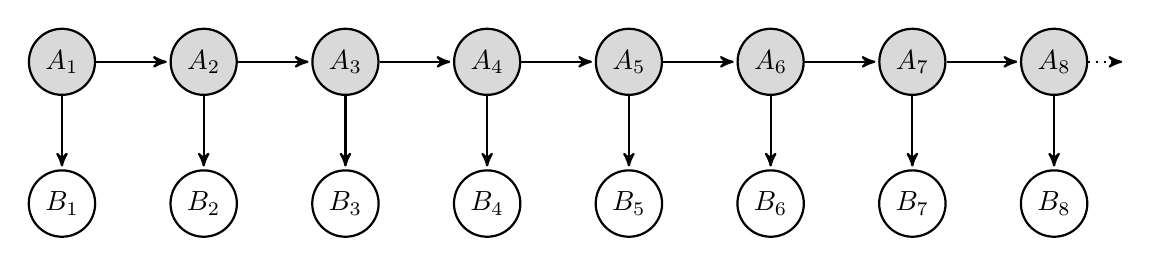
\begin{tikzpicture}[->, >=stealth',shorten >=1pt,auto, node distance=2cm, thick,main/.style={circle,draw}, x=1.8cm, y=1.8cm]
    % time
    \eat{
    \foreach \i in {1,...,4} {
        \node[rectangle, fill=gray!30] (t\i) at (\i,-1) {$\i$};
    }
    \node[rectangle, fill=gray!30] (t5) at (5,-1) {$1$};
    \node[rectangle, fill=gray!30] (t6) at (6,-1) {$2$};
    \node[rectangle, fill=gray!30] (t7) at (7,-1) {$3$};
    \node[rectangle, fill=gray!30] (t8) at (8,-1) {$4$};
    }
    % chords, notes
    \foreach \i in {1,...,8} {
        \node[main, fill=gray!30] (A\i) at (\i,-2) {$A_{\i}$};
        \node[main] (B\i) at (\i,-3) {$B_{\i}$};
    }
    \eat{
    \node[main] (A'2) at (1.5,-2.5) {$A'_{2}$};
    \node[main] (A'3) at (2.5,-2.5) {$A'_{3}$};
    \node[main] (A'4) at (3.5,-2.5) {$A'_{4}$};
    \node[main] (A'5) at (4.5,-2.5) {$A'_{5}$};
    \node[main] (A'6) at (5.5,-2.5) {$A'_{6}$};
    \node[main] (A'7) at (6.5,-2.5) {$A'_{7}$};
    \node[main] (A'8) at (7.5,-2.5) {$A'_{8}$};
    
    \node[main] (B'2) at (1.5,-3.5) {$B'_{2}$};
    \node[main] (B'3) at (2.5,-3.5) {$B'_{3}$};
    \node[main] (B'4) at (3.5,-3.5) {$B'_{4}$};
    \node[main] (B'5) at (4.5,-3.5) {$B'_{5}$};
    \node[main] (B'6) at (5.5,-3.5) {$B'_{6}$};
    \node[main] (B'7) at (6.5,-3.5) {$B'_{7}$};
    \node[main] (B'8) at (7.5,-3.5) {$B'_{8}$};
    
    
    
    \foreach \a in {A,B} {
    \draw (\a2) to (\a'2); \draw (\a1) to (\a'2);
    \draw (\a3) to (\a'3); \draw (\a2) to (\a'3);
    \draw (\a4) to (\a'4); \draw (\a3) to (\a'4);
    \draw (\a5) to (\a'5); \draw (\a4) to (\a'5);
    \draw (\a6) to (\a'6); \draw (\a5) to (\a'6);
    \draw (\a7) to (\a'7); \draw (\a6) to (\a'7);
    \draw (\a8) to (\a'8); \draw (\a7) to (\a'8);
    }
    }
    
    \foreach \i in {1,...,8} {
        \draw (A\i) to (B\i);
        %\draw (t\i) to (A\i);
    }
    
    \foreach \a in {A} {
        \draw (\a1) to (\a2);
        \draw (\a2) to (\a3);
        \draw (\a3) to (\a4);
        \draw (\a4) to (\a5);
        \draw (\a5) to (\a6);
        \draw (\a6) to (\a7);
        \draw (\a7) to (\a8);
    }
    %\draw[dotted] (t8) to (8.5,-1);
    \draw[dotted] (A8) to (8.5,-2);
    %\draw[dotted] (B8) to (8.5,-3);
\end{tikzpicture}}
\end{center}
\caption{Simple model 1}
\end{minipage}
\quad
\begin{minipage}{0.45\textwidth}
\begin{center}
\resizebox{\textwidth}{!}{
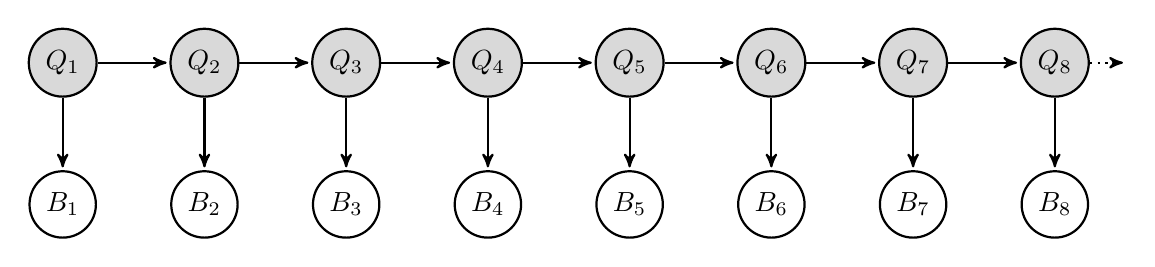
\begin{tikzpicture}[->, >=stealth',shorten >=1pt,auto, node distance=2cm, thick,main/.style={circle,draw}, x=1.8cm, y=1.8cm]
    % time
    \eat{
    \foreach \i in {1,...,4} {
        \node[rectangle, fill=gray!30] (t\i) at (\i,-1) {$\i$};
    }
    \node[rectangle, fill=gray!30] (t5) at (5,-1) {$1$};
    \node[rectangle, fill=gray!30] (t6) at (6,-1) {$2$};
    \node[rectangle, fill=gray!30] (t7) at (7,-1) {$3$};
    \node[rectangle, fill=gray!30] (t8) at (8,-1) {$4$};
    }
    % chords, notes
    \foreach \i in {1,...,8} {
        \node[main, fill=gray!30] (A\i) at (\i,-2) {$Q_{\i}$};
        \node[main] (B\i) at (\i,-3) {$B_{\i}$};
    }
    \eat{
    \node[main] (A'2) at (1.5,-2.5) {$A'_{2}$};
    \node[main] (A'3) at (2.5,-2.5) {$A'_{3}$};
    \node[main] (A'4) at (3.5,-2.5) {$A'_{4}$};
    \node[main] (A'5) at (4.5,-2.5) {$A'_{5}$};
    \node[main] (A'6) at (5.5,-2.5) {$A'_{6}$};
    \node[main] (A'7) at (6.5,-2.5) {$A'_{7}$};
    \node[main] (A'8) at (7.5,-2.5) {$A'_{8}$};
    
    \node[main] (B'2) at (1.5,-3.5) {$B'_{2}$};
    \node[main] (B'3) at (2.5,-3.5) {$B'_{3}$};
    \node[main] (B'4) at (3.5,-3.5) {$B'_{4}$};
    \node[main] (B'5) at (4.5,-3.5) {$B'_{5}$};
    \node[main] (B'6) at (5.5,-3.5) {$B'_{6}$};
    \node[main] (B'7) at (6.5,-3.5) {$B'_{7}$};
    \node[main] (B'8) at (7.5,-3.5) {$B'_{8}$};
    
    
    
    \foreach \a in {A,B} {
    \draw (\a2) to (\a'2); \draw (\a1) to (\a'2);
    \draw (\a3) to (\a'3); \draw (\a2) to (\a'3);
    \draw (\a4) to (\a'4); \draw (\a3) to (\a'4);
    \draw (\a5) to (\a'5); \draw (\a4) to (\a'5);
    \draw (\a6) to (\a'6); \draw (\a5) to (\a'6);
    \draw (\a7) to (\a'7); \draw (\a6) to (\a'7);
    \draw (\a8) to (\a'8); \draw (\a7) to (\a'8);
    }
    }
    
    \foreach \i in {1,...,8} {
        \draw (A\i) to (B\i);
        %\draw (t\i) to (A\i);
    }
    
    \foreach \a in {A} {
        \draw (\a1) to (\a2);
        \draw (\a2) to (\a3);
        \draw (\a3) to (\a4);
        \draw (\a4) to (\a5);
        \draw (\a5) to (\a6);
        \draw (\a6) to (\a7);
        \draw (\a7) to (\a8);
    }
    %\draw[dotted] (t8) to (8.5,-1);
    \draw[dotted] (A8) to (8.5,-2);
    %\draw[dotted] (B8) to (8.5,-3);
\end{tikzpicture}}
\end{center}
\caption{Simple model 2}
\end{minipage}
\end{figure}
\begin{figure}[ht]
\begin{minipage}{0.45\textwidth}
\begin{center}
\resizebox{\textwidth}{!}{
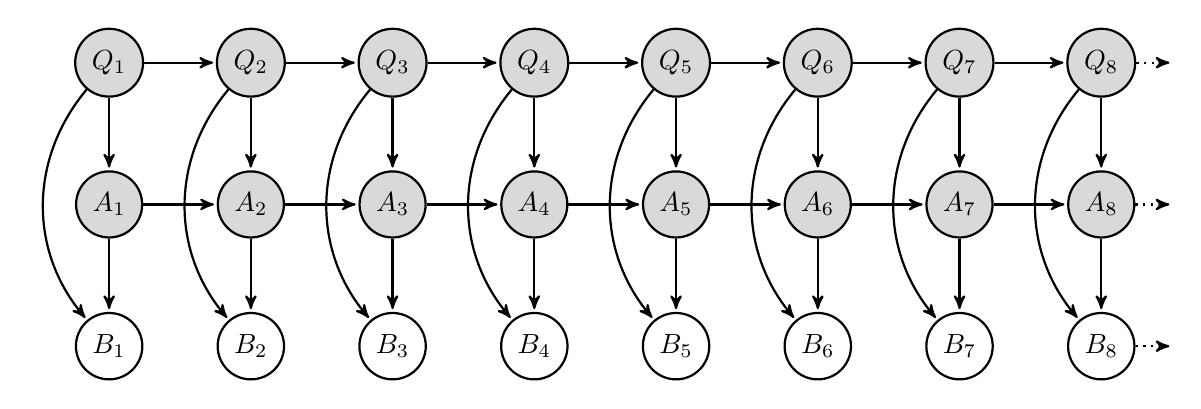
\begin{tikzpicture}[->, >=stealth',shorten >=1pt,auto, node distance=2cm, thick,main/.style={circle,draw}, x=1.8cm, y=1.8cm]
    % time
    \eat{
    \foreach \i in {1,...,4} {
        \node[rectangle, fill=gray!30] (t\i) at (\i,0) {$\i$};
    }
    \node[rectangle, fill=gray!30] (t5) at (5,0) {$1$};
    \node[rectangle, fill=gray!30] (t6) at (6,0) {$2$};
    \node[rectangle, fill=gray!30] (t7) at (7,0) {$3$};
    \node[rectangle, fill=gray!30] (t8) at (8,0) {$4$};
    }
    % chords, notes
    \foreach \i in {1,...,8} {
        \node[main, fill=gray!30] (Q\i) at (\i,-1) {$Q_{\i}$};
        \node[main, fill=gray!30] (A\i) at (\i,-2) {$A_{\i}$};
        \node[main] (B\i) at (\i,-3) {$B_{\i}$};
    }
    \eat{
    \foreach \i in {1,...,7} {
        \node[main] (A'\i) at (\i.5, -2.5) {$A'_{\i}$};
        \draw (A\i) to (A'\i);
    }
    
    \node[main] (A'2) at (1.5,-2.5) {$A'_{2}$};
    \node[main] (A'3) at (2.5,-2.5) {$A'_{3}$};
    \node[main] (A'4) at (3.5,-2.5) {$A'_{4}$};
    \node[main] (A'5) at (4.5,-2.5) {$A'_{5}$};
    \node[main] (A'6) at (5.5,-2.5) {$A'_{6}$};
    \node[main] (A'7) at (6.5,-2.5) {$A'_{7}$};
    \node[main] (A'8) at (7.5,-2.5) {$A'_{8}$};
    
    \node[main] (B'2) at (1.5,-3.5) {$B'_{2}$};
    \node[main] (B'3) at (2.5,-3.5) {$B'_{3}$};
    \node[main] (B'4) at (3.5,-3.5) {$B'_{4}$};
    \node[main] (B'5) at (4.5,-3.5) {$B'_{5}$};
    \node[main] (B'6) at (5.5,-3.5) {$B'_{6}$};
    \node[main] (B'7) at (6.5,-3.5) {$B'_{7}$};
    \node[main] (B'8) at (7.5,-3.5) {$B'_{8}$};
    
    \node[main] (C'2) at (1.5,-4.5) {$C'_{2}$};
    \node[main] (C'3) at (2.5,-4.5) {$C'_{3}$};
    \node[main] (C'4) at (3.5,-4.5) {$C'_{4}$};
    \node[main] (C'5) at (4.5,-4.5) {$C'_{5}$};
    \node[main] (C'6) at (5.5,-4.5) {$C'_{6}$};
    \node[main] (C'7) at (6.5,-4.5) {$C'_{7}$};
    \node[main] (C'8) at (7.5,-4.5) {$C'_{8}$};
    
    \node[main] (D'2) at (1.5,-5.5) {$D'_{2}$};
    \node[main] (D'3) at (2.5,-5.5) {$D'_{3}$};
    \node[main] (D'4) at (3.5,-5.5) {$D'_{4}$};
    \node[main] (D'5) at (4.5,-5.5) {$D'_{5}$};
    \node[main] (D'6) at (5.5,-5.5) {$D'_{6}$};
    \node[main] (D'7) at (6.5,-5.5) {$D'_{7}$};
    \node[main] (D'8) at (7.5,-5.5) {$D'_{8}$};
    }
    \eat{
    \draw (A2) to (A'1);
    \draw (A3) to (A'2);
    \draw (A4) to (A'3);
    \draw (A5) to (A'4);
    \draw (A6) to (A'5);
    \draw (A7) to (A'6);
    \draw (A8) to (A'7);
    }
    
    \eat{
    \foreach \i in {1,...,7} {
        \node[main] (B'\i) at (\i.5, -3.5) {$B'_{\i}$};
        \draw (B\i) to (B'\i);
    }
    }
    \eat{
    \draw (B2) to (B'1);
    \draw (B3) to (B'2);
    \draw (B4) to (B'3);
    \draw (B5) to (B'4);
    \draw (B6) to (B'5);
    \draw (B7) to (B'6);
    \draw (B8) to (B'7);
    }
    
    \eat{
    \foreach \i in {1,...,7} {
        \node[main] (C'\i) at (\i.5, -4.5) {$C'_{\i}$};
        \draw (C\i) to (C'\i);
    }
    
    \foreach \i in {1,...,7} {
        \node[main] (D'\i) at (\i.5, -5.5) {$D'_{\i}$};
        \draw (D\i) to (D'\i);
    }
    
    \foreach \a in {A,B} {
    \draw (\a2) to (\a'2); \draw (\a1) to (\a'2);
    \draw (\a3) to (\a'3); \draw (\a2) to (\a'3);
    \draw (\a4) to (\a'4); \draw (\a3) to (\a'4);
    \draw (\a5) to (\a'5); \draw (\a4) to (\a'5);
    \draw (\a6) to (\a'6); \draw (\a5) to (\a'6);
    \draw (\a7) to (\a'7); \draw (\a6) to (\a'7);
    \draw (\a8) to (\a'8); \draw (\a7) to (\a'8);
    }
    }
    \foreach \i in {1,...,8} {
        %\draw (t\i) to (Q\i);
        \draw (Q\i) to (A\i);
        \draw[bend right=40] (Q\i) to (B\i);
        %\draw[bend right=40] (Q\i) to (C\i);
        %\draw[bend right=40] (Q\i) to (D\i);
        \draw (A\i) to (B\i);
        %\draw[bend right=40] (A\i) to (C\i);
        
    }
    
    \foreach \a in {A,Q} {
        \draw (\a1) to (\a2);
        \draw (\a2) to (\a3);
        \draw (\a3) to (\a4);
        \draw (\a4) to (\a5);
        \draw (\a5) to (\a6);
        \draw (\a6) to (\a7);
        \draw (\a7) to (\a8);
    }
    %\draw[dotted] (t8) to (8.5,0);
    \draw[dotted] (A8) to (8.5,-2);
    \draw[dotted] (B8) to (8.5,-3);
    %\draw[dotted] (C8) to (8.5,-4);
    %\draw[dotted] (D8) to (8.5,-5);
    \draw[dotted] (Q8) to (8.5,-1);
\end{tikzpicture}}
\end{center}
\caption{Intermediate model 1}
\end{minipage}
\quad
\begin{minipage}{0.45\textwidth}
\resizebox{\textwidth}{!}{
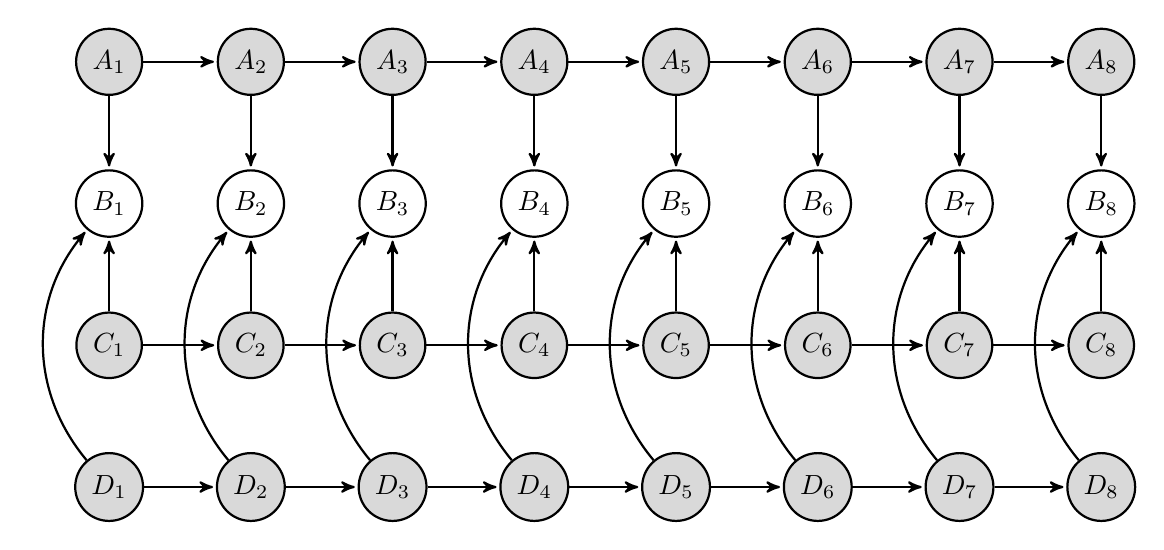
\begin{tikzpicture}[->, >=stealth',shorten >=1pt,auto, node distance=2cm, thick,main/.style={circle,draw}, x=1.8cm, y=1.8cm]
    % time
    \eat{
    \foreach \i in {1,...,4} {
        \node[rectangle, fill=gray!30] (t\i) at (\i,0) {$\i$};
    }
    \node[rectangle, fill=gray!30] (t5) at (5,0) {$1$};
    \node[rectangle, fill=gray!30] (t6) at (6,0) {$2$};
    \node[rectangle, fill=gray!30] (t7) at (7,0) {$3$};
    \node[rectangle, fill=gray!30] (t8) at (8,0) {$4$};
    }
    
    % chords, notes
    \foreach \i in {1,...,8} {
        %\node[main, fill=gray!30] (Q\i) at (\i,-1) {$Q_{\i}$};
        \node[main, fill=gray!30] (A\i) at (\i,-2) {$A_{\i}$};
        \node[main] (B\i) at (\i,-3) {$B_{\i}$};
        \node[main, fill=gray!30] (C\i) at (\i,-4) {$C_{\i}$};
        \node[main, fill=gray!30] (D\i) at (\i,-5) {$D_{\i}$};
    }
    \eat{
    \foreach \i in {1,...,7} {
        \node[main] (A'\i) at (\i.5, -2.5) {$A'_{\i}$};
        \draw (A\i) to (A'\i);
    }
    
    \node[main] (A'2) at (1.5,-2.5) {$A'_{2}$};
    \node[main] (A'3) at (2.5,-2.5) {$A'_{3}$};
    \node[main] (A'4) at (3.5,-2.5) {$A'_{4}$};
    \node[main] (A'5) at (4.5,-2.5) {$A'_{5}$};
    \node[main] (A'6) at (5.5,-2.5) {$A'_{6}$};
    \node[main] (A'7) at (6.5,-2.5) {$A'_{7}$};
    \node[main] (A'8) at (7.5,-2.5) {$A'_{8}$};
    
    \node[main] (B'2) at (1.5,-3.5) {$B'_{2}$};
    \node[main] (B'3) at (2.5,-3.5) {$B'_{3}$};
    \node[main] (B'4) at (3.5,-3.5) {$B'_{4}$};
    \node[main] (B'5) at (4.5,-3.5) {$B'_{5}$};
    \node[main] (B'6) at (5.5,-3.5) {$B'_{6}$};
    \node[main] (B'7) at (6.5,-3.5) {$B'_{7}$};
    \node[main] (B'8) at (7.5,-3.5) {$B'_{8}$};
    
    \node[main] (C'2) at (1.5,-4.5) {$C'_{2}$};
    \node[main] (C'3) at (2.5,-4.5) {$C'_{3}$};
    \node[main] (C'4) at (3.5,-4.5) {$C'_{4}$};
    \node[main] (C'5) at (4.5,-4.5) {$C'_{5}$};
    \node[main] (C'6) at (5.5,-4.5) {$C'_{6}$};
    \node[main] (C'7) at (6.5,-4.5) {$C'_{7}$};
    \node[main] (C'8) at (7.5,-4.5) {$C'_{8}$};
    
    \node[main] (D'2) at (1.5,-5.5) {$D'_{2}$};
    \node[main] (D'3) at (2.5,-5.5) {$D'_{3}$};
    \node[main] (D'4) at (3.5,-5.5) {$D'_{4}$};
    \node[main] (D'5) at (4.5,-5.5) {$D'_{5}$};
    \node[main] (D'6) at (5.5,-5.5) {$D'_{6}$};
    \node[main] (D'7) at (6.5,-5.5) {$D'_{7}$};
    \node[main] (D'8) at (7.5,-5.5) {$D'_{8}$};
    }
    \eat{
    \draw (A2) to (A'1);
    \draw (A3) to (A'2);
    \draw (A4) to (A'3);
    \draw (A5) to (A'4);
    \draw (A6) to (A'5);
    \draw (A7) to (A'6);
    \draw (A8) to (A'7);
    }
    
    \eat{
    \foreach \i in {1,...,7} {
        \node[main] (B'\i) at (\i.5, -3.5) {$B'_{\i}$};
        \draw (B\i) to (B'\i);
    }
    }
    \eat{
    \draw (B2) to (B'1);
    \draw (B3) to (B'2);
    \draw (B4) to (B'3);
    \draw (B5) to (B'4);
    \draw (B6) to (B'5);
    \draw (B7) to (B'6);
    \draw (B8) to (B'7);
    }
    
    \eat{
    \foreach \i in {1,...,7} {
        \node[main] (C'\i) at (\i.5, -4.5) {$C'_{\i}$};
        \draw (C\i) to (C'\i);
    }
    
    \foreach \i in {1,...,7} {
        \node[main] (D'\i) at (\i.5, -5.5) {$D'_{\i}$};
        \draw (D\i) to (D'\i);
    }
    
    \foreach \a in {A,B,C,D} {
    \draw (\a2) to (\a'2); \draw (\a1) to (\a'2);
    \draw (\a3) to (\a'3); \draw (\a2) to (\a'3);
    \draw (\a4) to (\a'4); \draw (\a3) to (\a'4);
    \draw (\a5) to (\a'5); \draw (\a4) to (\a'5);
    \draw (\a6) to (\a'6); \draw (\a5) to (\a'6);
    \draw (\a7) to (\a'7); \draw (\a6) to (\a'7);
    \draw (\a8) to (\a'8); \draw (\a7) to (\a'8);
    }
    }
    
    \foreach \i in {1,...,8} {
        %\draw (t\i) to (Q\i);
        %\draw[bend right=40] (Q\i) to (B\i);
        \draw (C\i) to (B\i);
        \draw[bend left=40] (D\i) to (B\i);
        %\draw[bend right=40] (Q\i) to (B\i);
        \draw (A\i) to (B\i);
        %\draw[bend right=40] (A\i) to (C\i);
        
    }
    
    \foreach \a in {A,C,D} {
        \draw (\a1) to (\a2);
        \draw (\a2) to (\a3);
        \draw (\a3) to (\a4);
        \draw (\a4) to (\a5);
        \draw (\a5) to (\a6);
        \draw (\a6) to (\a7);
        \draw (\a7) to (\a8);
    }
    \eat{
    \draw[dotted] (t8) to (8.5,0);
    \draw[dotted] (A8) to (8.5,-2);
    \draw[dotted] (B8) to (8.5,-3);
    \draw[dotted] (C8) to (8.5,-4);
    \draw[dotted] (D8) to (8.5,-5);
    \draw[dotted] (Q8) to (8.5,-1);
    }
\end{tikzpicture}}
\caption{Intermediate model 2}
\end{minipage}
\end{figure}
\begin{figure}[ht]
\begin{minipage}{.45\textwidth}
\begin{center}
\resizebox{\textwidth}{!}{
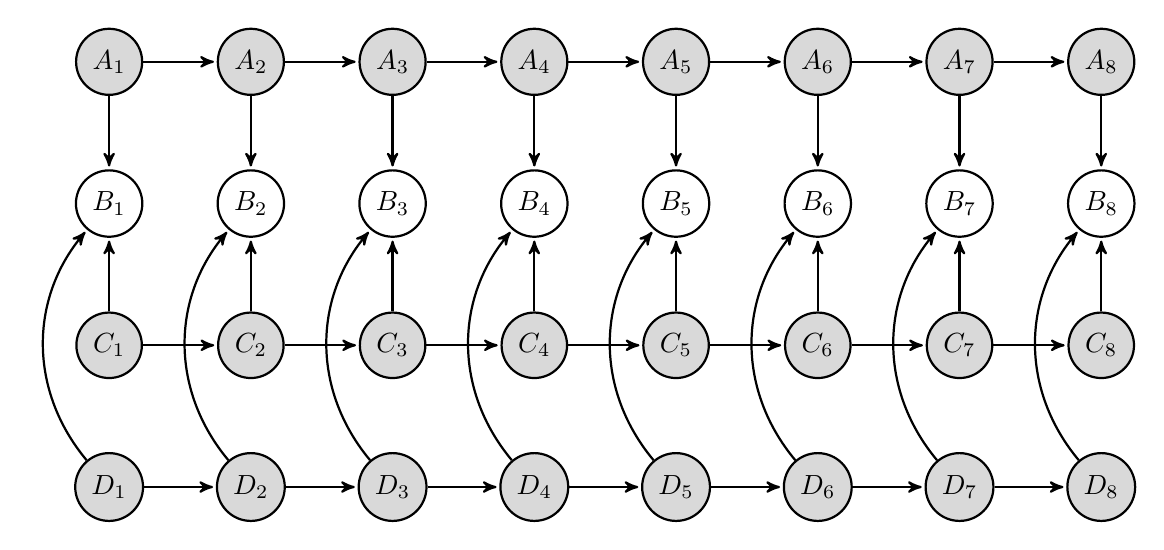
\begin{tikzpicture}[->, >=stealth',shorten >=1pt,auto, node distance=2cm, thick,main/.style={circle,draw}, x=1.8cm, y=1.8cm]
    % time
    \eat{
    \foreach \i in {1,...,4} {
        \node[rectangle, fill=gray!30] (t\i) at (\i,0) {$\i$};
    }
    \node[rectangle, fill=gray!30] (t5) at (5,0) {$1$};
    \node[rectangle, fill=gray!30] (t6) at (6,0) {$2$};
    \node[rectangle, fill=gray!30] (t7) at (7,0) {$3$};
    \node[rectangle, fill=gray!30] (t8) at (8,0) {$4$};
    }
    
    % chords, notes
    \foreach \i in {1,...,8} {
        %\node[main, fill=gray!30] (Q\i) at (\i,-1) {$Q_{\i}$};
        \node[main, fill=gray!30] (A\i) at (\i,-2) {$A_{\i}$};
        \node[main] (B\i) at (\i,-3) {$B_{\i}$};
        \node[main, fill=gray!30] (C\i) at (\i,-4) {$C_{\i}$};
        \node[main, fill=gray!30] (D\i) at (\i,-5) {$D_{\i}$};
    }
    \eat{
    \foreach \i in {1,...,7} {
        \node[main] (A'\i) at (\i.5, -2.5) {$A'_{\i}$};
        \draw (A\i) to (A'\i);
    }
    
    \node[main] (A'2) at (1.5,-2.5) {$A'_{2}$};
    \node[main] (A'3) at (2.5,-2.5) {$A'_{3}$};
    \node[main] (A'4) at (3.5,-2.5) {$A'_{4}$};
    \node[main] (A'5) at (4.5,-2.5) {$A'_{5}$};
    \node[main] (A'6) at (5.5,-2.5) {$A'_{6}$};
    \node[main] (A'7) at (6.5,-2.5) {$A'_{7}$};
    \node[main] (A'8) at (7.5,-2.5) {$A'_{8}$};
    
    \node[main] (B'2) at (1.5,-3.5) {$B'_{2}$};
    \node[main] (B'3) at (2.5,-3.5) {$B'_{3}$};
    \node[main] (B'4) at (3.5,-3.5) {$B'_{4}$};
    \node[main] (B'5) at (4.5,-3.5) {$B'_{5}$};
    \node[main] (B'6) at (5.5,-3.5) {$B'_{6}$};
    \node[main] (B'7) at (6.5,-3.5) {$B'_{7}$};
    \node[main] (B'8) at (7.5,-3.5) {$B'_{8}$};
    
    \node[main] (C'2) at (1.5,-4.5) {$C'_{2}$};
    \node[main] (C'3) at (2.5,-4.5) {$C'_{3}$};
    \node[main] (C'4) at (3.5,-4.5) {$C'_{4}$};
    \node[main] (C'5) at (4.5,-4.5) {$C'_{5}$};
    \node[main] (C'6) at (5.5,-4.5) {$C'_{6}$};
    \node[main] (C'7) at (6.5,-4.5) {$C'_{7}$};
    \node[main] (C'8) at (7.5,-4.5) {$C'_{8}$};
    
    \node[main] (D'2) at (1.5,-5.5) {$D'_{2}$};
    \node[main] (D'3) at (2.5,-5.5) {$D'_{3}$};
    \node[main] (D'4) at (3.5,-5.5) {$D'_{4}$};
    \node[main] (D'5) at (4.5,-5.5) {$D'_{5}$};
    \node[main] (D'6) at (5.5,-5.5) {$D'_{6}$};
    \node[main] (D'7) at (6.5,-5.5) {$D'_{7}$};
    \node[main] (D'8) at (7.5,-5.5) {$D'_{8}$};
    }
    \eat{
    \draw (A2) to (A'1);
    \draw (A3) to (A'2);
    \draw (A4) to (A'3);
    \draw (A5) to (A'4);
    \draw (A6) to (A'5);
    \draw (A7) to (A'6);
    \draw (A8) to (A'7);
    }
    
    \eat{
    \foreach \i in {1,...,7} {
        \node[main] (B'\i) at (\i.5, -3.5) {$B'_{\i}$};
        \draw (B\i) to (B'\i);
    }
    }
    \eat{
    \draw (B2) to (B'1);
    \draw (B3) to (B'2);
    \draw (B4) to (B'3);
    \draw (B5) to (B'4);
    \draw (B6) to (B'5);
    \draw (B7) to (B'6);
    \draw (B8) to (B'7);
    }
    
    \eat{
    \foreach \i in {1,...,7} {
        \node[main] (C'\i) at (\i.5, -4.5) {$C'_{\i}$};
        \draw (C\i) to (C'\i);
    }
    
    \foreach \i in {1,...,7} {
        \node[main] (D'\i) at (\i.5, -5.5) {$D'_{\i}$};
        \draw (D\i) to (D'\i);
    }
    
    \foreach \a in {A,B,C,D} {
    \draw (\a2) to (\a'2); \draw (\a1) to (\a'2);
    \draw (\a3) to (\a'3); \draw (\a2) to (\a'3);
    \draw (\a4) to (\a'4); \draw (\a3) to (\a'4);
    \draw (\a5) to (\a'5); \draw (\a4) to (\a'5);
    \draw (\a6) to (\a'6); \draw (\a5) to (\a'6);
    \draw (\a7) to (\a'7); \draw (\a6) to (\a'7);
    \draw (\a8) to (\a'8); \draw (\a7) to (\a'8);
    }
    }
    
    \foreach \i in {1,...,8} {
        %\draw (t\i) to (Q\i);
        %\draw[bend right=40] (Q\i) to (B\i);
        \draw (C\i) to (B\i);
        \draw[bend left=40] (D\i) to (B\i);
        %\draw[bend right=40] (Q\i) to (B\i);
        \draw (A\i) to (B\i);
        %\draw[bend right=40] (A\i) to (C\i);
        
    }
    
    \foreach \a in {A,C,D} {
        \draw (\a1) to (\a2);
        \draw (\a2) to (\a3);
        \draw (\a3) to (\a4);
        \draw (\a4) to (\a5);
        \draw (\a5) to (\a6);
        \draw (\a6) to (\a7);
        \draw (\a7) to (\a8);
    }
    \eat{
    \draw[dotted] (t8) to (8.5,0);
    \draw[dotted] (A8) to (8.5,-2);
    \draw[dotted] (B8) to (8.5,-3);
    \draw[dotted] (C8) to (8.5,-4);
    \draw[dotted] (D8) to (8.5,-5);
    \draw[dotted] (Q8) to (8.5,-1);
    }
\end{tikzpicture}}
\end{center}
\caption{Intermediate model 2}
\end{minipage}
\qquad
\begin{minipage}{.45\textwidth}
\begin{center}
\resizebox{\textwidth}{!}{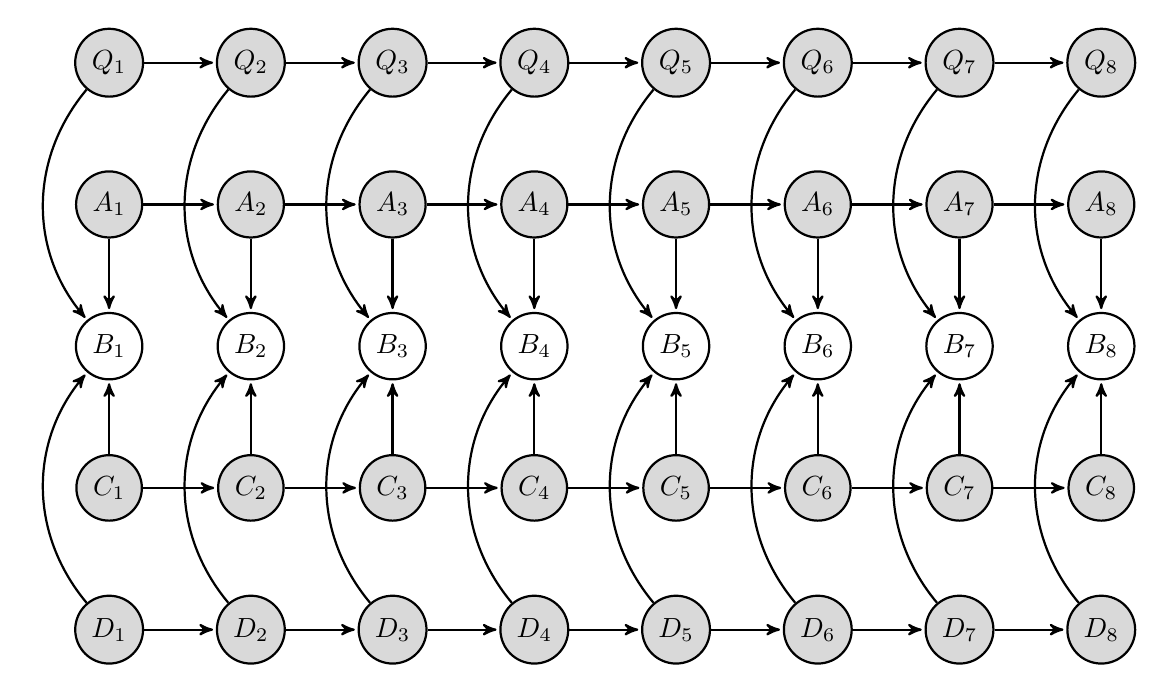
\begin{tikzpicture}[->, >=stealth',shorten >=1pt,auto, node distance=2cm, thick,main/.style={circle,draw}, x=1.8cm, y=1.8cm]
    % time
    \eat{
    \foreach \i in {1,...,4} {
        \node[rectangle, fill=gray!30] (t\i) at (\i,0) {$\i$};
    }
    \node[rectangle, fill=gray!30] (t5) at (5,0) {$1$};
    \node[rectangle, fill=gray!30] (t6) at (6,0) {$2$};
    \node[rectangle, fill=gray!30] (t7) at (7,0) {$3$};
    \node[rectangle, fill=gray!30] (t8) at (8,0) {$4$};
    }
    
    % chords, notes
    \foreach \i in {1,...,8} {
        \node[main, fill=gray!30] (Q\i) at (\i,-1) {$Q_{\i}$};
        \node[main, fill=gray!30] (A\i) at (\i,-2) {$A_{\i}$};
        \node[main] (B\i) at (\i,-3) {$B_{\i}$};
        \node[main, fill=gray!30] (C\i) at (\i,-4) {$C_{\i}$};
        \node[main, fill=gray!30] (D\i) at (\i,-5) {$D_{\i}$};
    }
    \eat{
    \foreach \i in {1,...,7} {
        \node[main] (A'\i) at (\i.5, -2.5) {$A'_{\i}$};
        \draw (A\i) to (A'\i);
    }
    
    \node[main] (A'2) at (1.5,-2.5) {$A'_{2}$};
    \node[main] (A'3) at (2.5,-2.5) {$A'_{3}$};
    \node[main] (A'4) at (3.5,-2.5) {$A'_{4}$};
    \node[main] (A'5) at (4.5,-2.5) {$A'_{5}$};
    \node[main] (A'6) at (5.5,-2.5) {$A'_{6}$};
    \node[main] (A'7) at (6.5,-2.5) {$A'_{7}$};
    \node[main] (A'8) at (7.5,-2.5) {$A'_{8}$};
    
    \node[main] (B'2) at (1.5,-3.5) {$B'_{2}$};
    \node[main] (B'3) at (2.5,-3.5) {$B'_{3}$};
    \node[main] (B'4) at (3.5,-3.5) {$B'_{4}$};
    \node[main] (B'5) at (4.5,-3.5) {$B'_{5}$};
    \node[main] (B'6) at (5.5,-3.5) {$B'_{6}$};
    \node[main] (B'7) at (6.5,-3.5) {$B'_{7}$};
    \node[main] (B'8) at (7.5,-3.5) {$B'_{8}$};
    
    \node[main] (C'2) at (1.5,-4.5) {$C'_{2}$};
    \node[main] (C'3) at (2.5,-4.5) {$C'_{3}$};
    \node[main] (C'4) at (3.5,-4.5) {$C'_{4}$};
    \node[main] (C'5) at (4.5,-4.5) {$C'_{5}$};
    \node[main] (C'6) at (5.5,-4.5) {$C'_{6}$};
    \node[main] (C'7) at (6.5,-4.5) {$C'_{7}$};
    \node[main] (C'8) at (7.5,-4.5) {$C'_{8}$};
    
    \node[main] (D'2) at (1.5,-5.5) {$D'_{2}$};
    \node[main] (D'3) at (2.5,-5.5) {$D'_{3}$};
    \node[main] (D'4) at (3.5,-5.5) {$D'_{4}$};
    \node[main] (D'5) at (4.5,-5.5) {$D'_{5}$};
    \node[main] (D'6) at (5.5,-5.5) {$D'_{6}$};
    \node[main] (D'7) at (6.5,-5.5) {$D'_{7}$};
    \node[main] (D'8) at (7.5,-5.5) {$D'_{8}$};
    }
    \eat{
    \draw (A2) to (A'1);
    \draw (A3) to (A'2);
    \draw (A4) to (A'3);
    \draw (A5) to (A'4);
    \draw (A6) to (A'5);
    \draw (A7) to (A'6);
    \draw (A8) to (A'7);
    }
    
    \eat{
    \foreach \i in {1,...,7} {
        \node[main] (B'\i) at (\i.5, -3.5) {$B'_{\i}$};
        \draw (B\i) to (B'\i);
    }
    }
    \eat{
    \draw (B2) to (B'1);
    \draw (B3) to (B'2);
    \draw (B4) to (B'3);
    \draw (B5) to (B'4);
    \draw (B6) to (B'5);
    \draw (B7) to (B'6);
    \draw (B8) to (B'7);
    }
    
    \eat{
    \foreach \i in {1,...,7} {
        \node[main] (C'\i) at (\i.5, -4.5) {$C'_{\i}$};
        \draw (C\i) to (C'\i);
    }
    
    \foreach \i in {1,...,7} {
        \node[main] (D'\i) at (\i.5, -5.5) {$D'_{\i}$};
        \draw (D\i) to (D'\i);
    }
    
    \foreach \a in {A,B,C,D} {
    \draw (\a2) to (\a'2); \draw (\a1) to (\a'2);
    \draw (\a3) to (\a'3); \draw (\a2) to (\a'3);
    \draw (\a4) to (\a'4); \draw (\a3) to (\a'4);
    \draw (\a5) to (\a'5); \draw (\a4) to (\a'5);
    \draw (\a6) to (\a'6); \draw (\a5) to (\a'6);
    \draw (\a7) to (\a'7); \draw (\a6) to (\a'7);
    \draw (\a8) to (\a'8); \draw (\a7) to (\a'8);
    }
    }
    
    \foreach \i in {1,...,8} {
        %\draw (t\i) to (Q\i);
        \draw[bend right=40] (Q\i) to (B\i);
        \draw (C\i) to (B\i);
        \draw[bend left=40] (D\i) to (B\i);
        %\draw[bend right=40] (Q\i) to (B\i);
        \draw (A\i) to (B\i);
        %\draw[bend right=40] (A\i) to (C\i);
        
    }
    
    \foreach \a in {A,C,D,Q} {
        \draw (\a1) to (\a2);
        \draw (\a2) to (\a3);
        \draw (\a3) to (\a4);
        \draw (\a4) to (\a5);
        \draw (\a5) to (\a6);
        \draw (\a6) to (\a7);
        \draw (\a7) to (\a8);
    }
    \eat{
    \draw[dotted] (t8) to (8.5,0);
    \draw[dotted] (A8) to (8.5,-2);
    \draw[dotted] (B8) to (8.5,-3);
    \draw[dotted] (C8) to (8.5,-4);
    \draw[dotted] (D8) to (8.5,-5);
    \draw[dotted] (Q8) to (8.5,-1);
    }
\end{tikzpicture}}
\end{center}
\caption{Intermediate model 3}
\end{minipage}
\end{figure}



\eat{
\begin{figure}[ht]
\begin{center}
\resizebox{0.5\textwidth}{!}{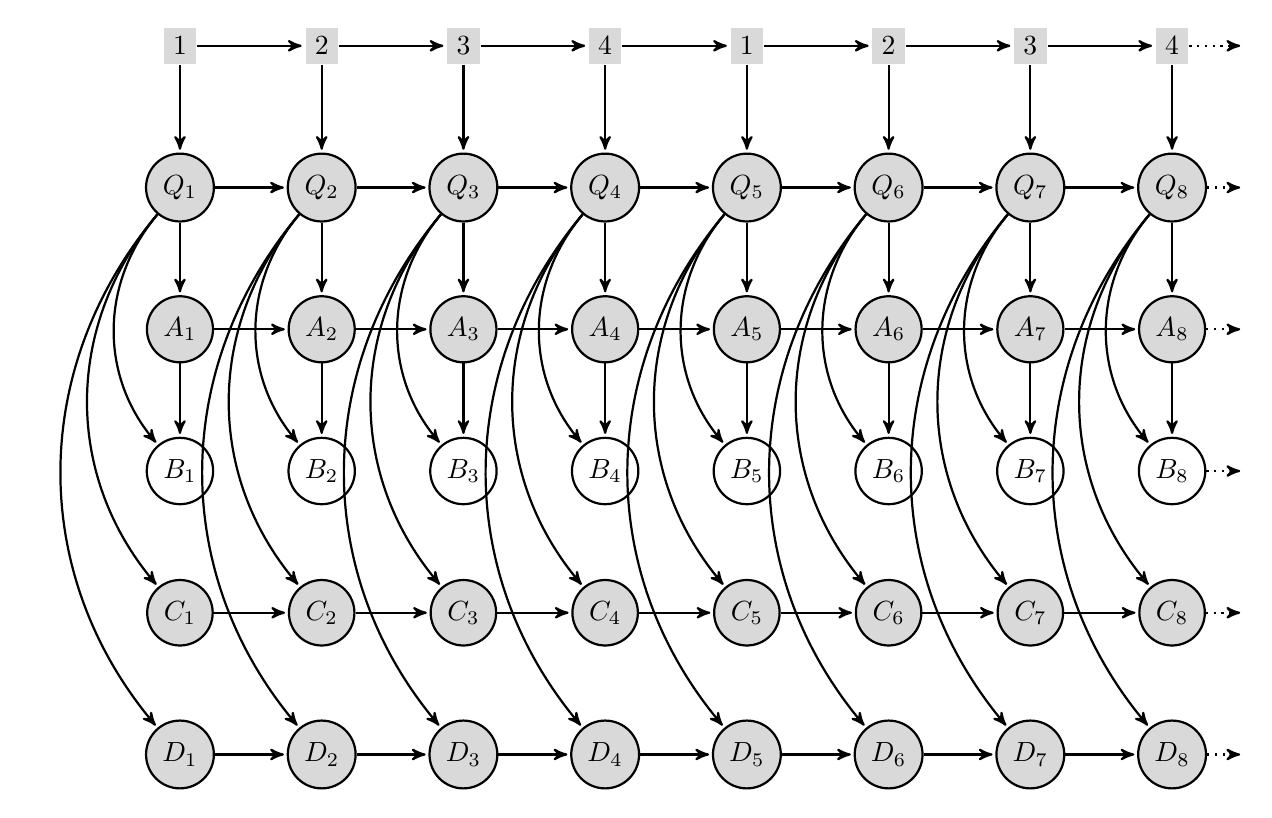
\begin{tikzpicture}[->, >=stealth',shorten >=1pt,auto, node distance=2cm, thick,main/.style={circle,draw}, x=1.8cm, y=1.8cm]
    % time
    \foreach \i in {1,...,4} {
        \node[rectangle, fill=gray!30] (t\i) at (\i,0) {$\i$};
    }
    \node[rectangle, fill=gray!30] (t5) at (5,0) {$1$};
    \node[rectangle, fill=gray!30] (t6) at (6,0) {$2$};
    \node[rectangle, fill=gray!30] (t7) at (7,0) {$3$};
    \node[rectangle, fill=gray!30] (t8) at (8,0) {$4$};
    
    % chords, notes
    \foreach \i in {1,...,8} {
        \node[main, fill=gray!30] (Q\i) at (\i,-1) {$Q_{\i}$};
        \node[main, fill=gray!30] (A\i) at (\i,-2) {$A_{\i}$};
        \node[main] (B\i) at (\i,-3) {$B_{\i}$};
        \node[main, fill=gray!30] (C\i) at (\i,-4) {$C_{\i}$};
        \node[main, fill=gray!30] (D\i) at (\i,-5) {$D_{\i}$};
    }
    \eat{
    \foreach \i in {1,...,7} {
        \node[main] (A'\i) at (\i.5, -2.5) {$A'_{\i}$};
        \draw (A\i) to (A'\i);
    }
    
    \node[main] (A'2) at (1.5,-2.5) {$A'_{2}$};
    \node[main] (A'3) at (2.5,-2.5) {$A'_{3}$};
    \node[main] (A'4) at (3.5,-2.5) {$A'_{4}$};
    \node[main] (A'5) at (4.5,-2.5) {$A'_{5}$};
    \node[main] (A'6) at (5.5,-2.5) {$A'_{6}$};
    \node[main] (A'7) at (6.5,-2.5) {$A'_{7}$};
    \node[main] (A'8) at (7.5,-2.5) {$A'_{8}$};
    
    \node[main] (B'2) at (1.5,-3.5) {$B'_{2}$};
    \node[main] (B'3) at (2.5,-3.5) {$B'_{3}$};
    \node[main] (B'4) at (3.5,-3.5) {$B'_{4}$};
    \node[main] (B'5) at (4.5,-3.5) {$B'_{5}$};
    \node[main] (B'6) at (5.5,-3.5) {$B'_{6}$};
    \node[main] (B'7) at (6.5,-3.5) {$B'_{7}$};
    \node[main] (B'8) at (7.5,-3.5) {$B'_{8}$};
    
    \node[main] (C'2) at (1.5,-4.5) {$C'_{2}$};
    \node[main] (C'3) at (2.5,-4.5) {$C'_{3}$};
    \node[main] (C'4) at (3.5,-4.5) {$C'_{4}$};
    \node[main] (C'5) at (4.5,-4.5) {$C'_{5}$};
    \node[main] (C'6) at (5.5,-4.5) {$C'_{6}$};
    \node[main] (C'7) at (6.5,-4.5) {$C'_{7}$};
    \node[main] (C'8) at (7.5,-4.5) {$C'_{8}$};
    
    \node[main] (D'2) at (1.5,-5.5) {$D'_{2}$};
    \node[main] (D'3) at (2.5,-5.5) {$D'_{3}$};
    \node[main] (D'4) at (3.5,-5.5) {$D'_{4}$};
    \node[main] (D'5) at (4.5,-5.5) {$D'_{5}$};
    \node[main] (D'6) at (5.5,-5.5) {$D'_{6}$};
    \node[main] (D'7) at (6.5,-5.5) {$D'_{7}$};
    \node[main] (D'8) at (7.5,-5.5) {$D'_{8}$};
    }
    \eat{
    \draw (A2) to (A'1);
    \draw (A3) to (A'2);
    \draw (A4) to (A'3);
    \draw (A5) to (A'4);
    \draw (A6) to (A'5);
    \draw (A7) to (A'6);
    \draw (A8) to (A'7);
    }
    
    \eat{
    \foreach \i in {1,...,7} {
        \node[main] (B'\i) at (\i.5, -3.5) {$B'_{\i}$};
        \draw (B\i) to (B'\i);
    }
    }
    \eat{
    \draw (B2) to (B'1);
    \draw (B3) to (B'2);
    \draw (B4) to (B'3);
    \draw (B5) to (B'4);
    \draw (B6) to (B'5);
    \draw (B7) to (B'6);
    \draw (B8) to (B'7);
    }
    
    \eat{
    \foreach \i in {1,...,7} {
        \node[main] (C'\i) at (\i.5, -4.5) {$C'_{\i}$};
        \draw (C\i) to (C'\i);
    }
    
    \foreach \i in {1,...,7} {
        \node[main] (D'\i) at (\i.5, -5.5) {$D'_{\i}$};
        \draw (D\i) to (D'\i);
    }
    }
    \eat{
    \foreach \a in {A,B,C,D} {
    \draw (\a2) to (\a'2); \draw (\a1) to (\a'2);
    \draw (\a3) to (\a'3); \draw (\a2) to (\a'3);
    \draw (\a4) to (\a'4); \draw (\a3) to (\a'4);
    \draw (\a5) to (\a'5); \draw (\a4) to (\a'5);
    \draw (\a6) to (\a'6); \draw (\a5) to (\a'6);
    \draw (\a7) to (\a'7); \draw (\a6) to (\a'7);
    \draw (\a8) to (\a'8); \draw (\a7) to (\a'8);
    }
    }
    
    \foreach \i in {1,...,8} {
        \draw (t\i) to (Q\i);
        \draw (Q\i) to (A\i);
        \draw[bend right=40] (Q\i) to (B\i);
        \draw[bend right=40] (Q\i) to (C\i);
        \draw[bend right=40] (Q\i) to (D\i);
        \draw (A\i) to (B\i);
        %\draw[bend right=40] (A\i) to (C\i);
        
    }
    
    \foreach \a in {A,C,D,Q, t} {
        \draw (\a1) to (\a2);
        \draw (\a2) to (\a3);
        \draw (\a3) to (\a4);
        \draw (\a4) to (\a5);
        \draw (\a5) to (\a6);
        \draw (\a6) to (\a7);
        \draw (\a7) to (\a8);
    }
    \draw[dotted] (t8) to (8.5,0);
    \draw[dotted] (A8) to (8.5,-2);
    \draw[dotted] (B8) to (8.5,-3);
    \draw[dotted] (C8) to (8.5,-4);
    \draw[dotted] (D8) to (8.5,-5);
    \draw[dotted] (Q8) to (8.5,-1);
\end{tikzpicture}}
\end{center}
\caption{Complex model 1}
\end{figure}
}



\begin{figure}[ht]
\begin{minipage}{.45\textwidth}
\begin{center}
\resizebox{\textwidth}{!}{
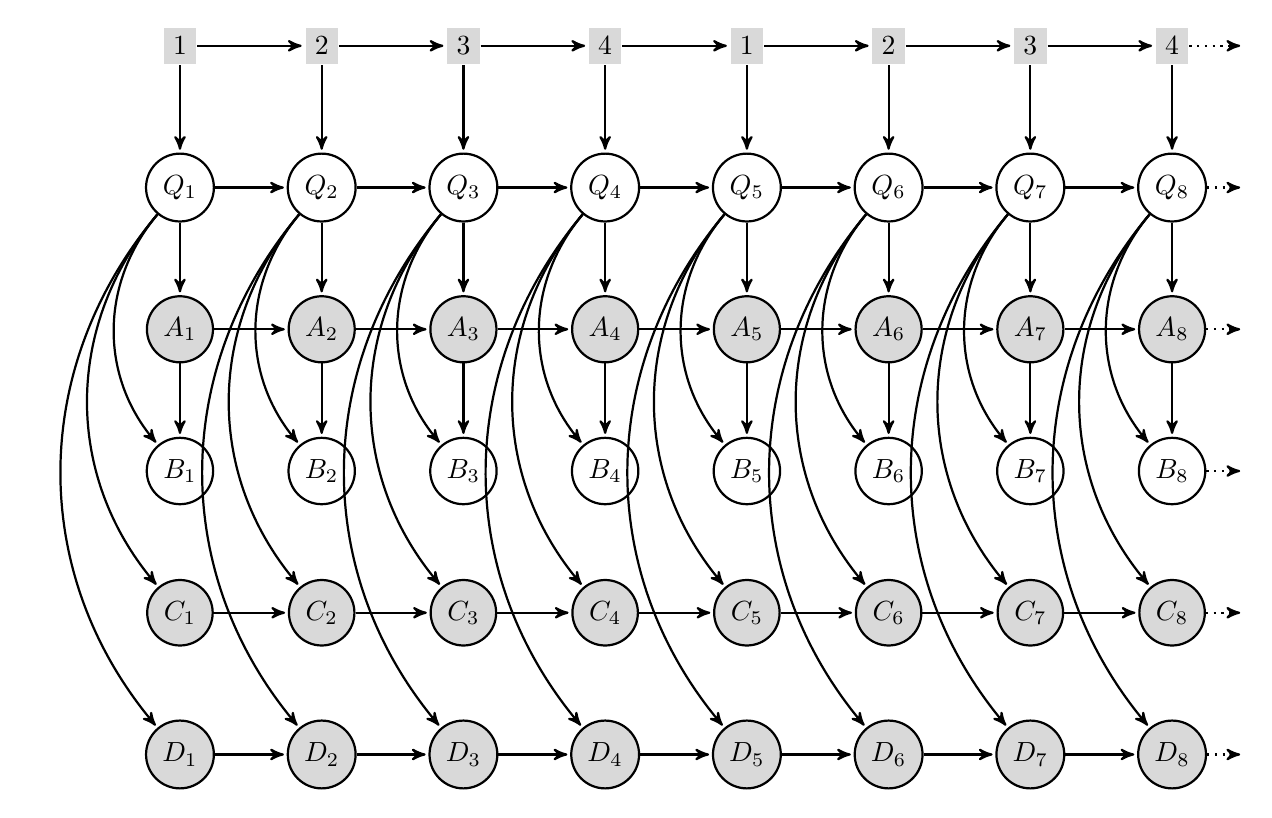
\begin{tikzpicture}[->, >=stealth',shorten >=1pt,auto, node distance=2cm, thick,main/.style={circle,draw}, x=1.8cm, y=1.8cm]
    % time
    \foreach \i in {1,...,4} {
        \node[rectangle, fill=gray!30] (t\i) at (\i,0) {$\i$};
    }
    \node[rectangle, fill=gray!30] (t5) at (5,0) {$1$};
    \node[rectangle, fill=gray!30] (t6) at (6,0) {$2$};
    \node[rectangle, fill=gray!30] (t7) at (7,0) {$3$};
    \node[rectangle, fill=gray!30] (t8) at (8,0) {$4$};
    
    % chords, notes
    \foreach \i in {1,...,8} {
        \node[main] (Q\i) at (\i,-1) {$Q_{\i}$};
        \node[main, fill=gray!30] (A\i) at (\i,-2) {$A_{\i}$};
        \node[main] (B\i) at (\i,-3) {$B_{\i}$};
        \node[main, fill=gray!30] (C\i) at (\i,-4) {$C_{\i}$};
        \node[main, fill=gray!30] (D\i) at (\i,-5) {$D_{\i}$};
    }
    \eat{
    \foreach \i in {1,...,7} {
        \node[main] (A'\i) at (\i.5, -2.5) {$A'_{\i}$};
        \draw (A\i) to (A'\i);
    }
    
    \node[main] (A'2) at (1.5,-2.5) {$A'_{2}$};
    \node[main] (A'3) at (2.5,-2.5) {$A'_{3}$};
    \node[main] (A'4) at (3.5,-2.5) {$A'_{4}$};
    \node[main] (A'5) at (4.5,-2.5) {$A'_{5}$};
    \node[main] (A'6) at (5.5,-2.5) {$A'_{6}$};
    \node[main] (A'7) at (6.5,-2.5) {$A'_{7}$};
    \node[main] (A'8) at (7.5,-2.5) {$A'_{8}$};
    
    \node[main] (B'2) at (1.5,-3.5) {$B'_{2}$};
    \node[main] (B'3) at (2.5,-3.5) {$B'_{3}$};
    \node[main] (B'4) at (3.5,-3.5) {$B'_{4}$};
    \node[main] (B'5) at (4.5,-3.5) {$B'_{5}$};
    \node[main] (B'6) at (5.5,-3.5) {$B'_{6}$};
    \node[main] (B'7) at (6.5,-3.5) {$B'_{7}$};
    \node[main] (B'8) at (7.5,-3.5) {$B'_{8}$};
    
    \node[main] (C'2) at (1.5,-4.5) {$C'_{2}$};
    \node[main] (C'3) at (2.5,-4.5) {$C'_{3}$};
    \node[main] (C'4) at (3.5,-4.5) {$C'_{4}$};
    \node[main] (C'5) at (4.5,-4.5) {$C'_{5}$};
    \node[main] (C'6) at (5.5,-4.5) {$C'_{6}$};
    \node[main] (C'7) at (6.5,-4.5) {$C'_{7}$};
    \node[main] (C'8) at (7.5,-4.5) {$C'_{8}$};
    
    \node[main] (D'2) at (1.5,-5.5) {$D'_{2}$};
    \node[main] (D'3) at (2.5,-5.5) {$D'_{3}$};
    \node[main] (D'4) at (3.5,-5.5) {$D'_{4}$};
    \node[main] (D'5) at (4.5,-5.5) {$D'_{5}$};
    \node[main] (D'6) at (5.5,-5.5) {$D'_{6}$};
    \node[main] (D'7) at (6.5,-5.5) {$D'_{7}$};
    \node[main] (D'8) at (7.5,-5.5) {$D'_{8}$};
    }
    \eat{
    \draw (A2) to (A'1);
    \draw (A3) to (A'2);
    \draw (A4) to (A'3);
    \draw (A5) to (A'4);
    \draw (A6) to (A'5);
    \draw (A7) to (A'6);
    \draw (A8) to (A'7);
    }
    
    \eat{
    \foreach \i in {1,...,7} {
        \node[main] (B'\i) at (\i.5, -3.5) {$B'_{\i}$};
        \draw (B\i) to (B'\i);
    }
    }
    \eat{
    \draw (B2) to (B'1);
    \draw (B3) to (B'2);
    \draw (B4) to (B'3);
    \draw (B5) to (B'4);
    \draw (B6) to (B'5);
    \draw (B7) to (B'6);
    \draw (B8) to (B'7);
    }
    
    \eat{
    \foreach \i in {1,...,7} {
        \node[main] (C'\i) at (\i.5, -4.5) {$C'_{\i}$};
        \draw (C\i) to (C'\i);
    }
    
    \foreach \i in {1,...,7} {
        \node[main] (D'\i) at (\i.5, -5.5) {$D'_{\i}$};
        \draw (D\i) to (D'\i);
    }
    }
    \eat{
    \foreach \a in {A,B,C,D} {
    \draw (\a2) to (\a'2); \draw (\a1) to (\a'2);
    \draw (\a3) to (\a'3); \draw (\a2) to (\a'3);
    \draw (\a4) to (\a'4); \draw (\a3) to (\a'4);
    \draw (\a5) to (\a'5); \draw (\a4) to (\a'5);
    \draw (\a6) to (\a'6); \draw (\a5) to (\a'6);
    \draw (\a7) to (\a'7); \draw (\a6) to (\a'7);
    \draw (\a8) to (\a'8); \draw (\a7) to (\a'8);
    }
    }
    
    \foreach \i in {1,...,8} {
        \draw (t\i) to (Q\i);
        \draw (Q\i) to (A\i);
        \draw[bend right=40] (Q\i) to (B\i);
        \draw[bend right=40] (Q\i) to (C\i);
        \draw[bend right=40] (Q\i) to (D\i);
        \draw (A\i) to (B\i);
        %\draw[bend right=40] (A\i) to (C\i);
        
    }
    
    \foreach \a in {A,C,D,Q, t} {
        \draw (\a1) to (\a2);
        \draw (\a2) to (\a3);
        \draw (\a3) to (\a4);
        \draw (\a4) to (\a5);
        \draw (\a5) to (\a6);
        \draw (\a6) to (\a7);
        \draw (\a7) to (\a8);
    }
    \draw[dotted] (t8) to (8.5,0);
    \draw[dotted] (A8) to (8.5,-2);
    \draw[dotted] (B8) to (8.5,-3);
    \draw[dotted] (C8) to (8.5,-4);
    \draw[dotted] (D8) to (8.5,-5);
    \draw[dotted] (Q8) to (8.5,-1);
\end{tikzpicture}}
\end{center}
\caption{Viterbi4}
\end{minipage}
\quad
\begin{minipage}{.45\textwidth}
\begin{center}
\resizebox{\textwidth}{!}{
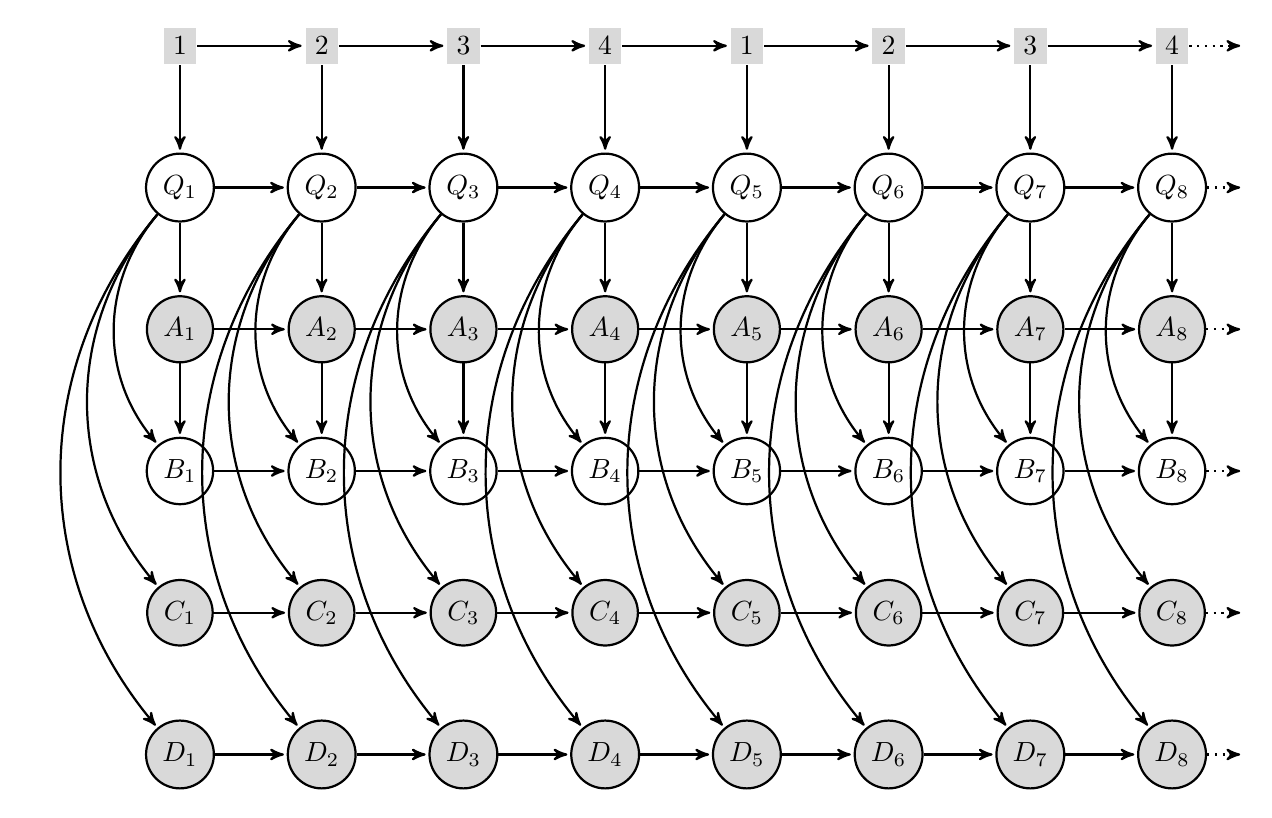
\begin{tikzpicture}[->, >=stealth',shorten >=1pt,auto, node distance=2cm, thick,main/.style={circle,draw}, x=1.8cm, y=1.8cm]
    % time
    \foreach \i in {1,...,4} {
        \node[rectangle, fill=gray!30] (t\i) at (\i,0) {$\i$};
    }
    \node[rectangle, fill=gray!30] (t5) at (5,0) {$1$};
    \node[rectangle, fill=gray!30] (t6) at (6,0) {$2$};
    \node[rectangle, fill=gray!30] (t7) at (7,0) {$3$};
    \node[rectangle, fill=gray!30] (t8) at (8,0) {$4$};
    
    % chords, notes
    \foreach \i in {1,...,8} {
        \node[main] (Q\i) at (\i,-1) {$Q_{\i}$};
        \node[main, fill=gray!30] (A\i) at (\i,-2) {$A_{\i}$};
        \node[main] (B\i) at (\i,-3) {$B_{\i}$};
        \node[main, fill=gray!30] (C\i) at (\i,-4) {$C_{\i}$};
        \node[main, fill=gray!30] (D\i) at (\i,-5) {$D_{\i}$};
    }
    \eat{
    \foreach \i in {1,...,7} {
        \node[main] (A'\i) at (\i.5, -2.5) {$A'_{\i}$};
        \draw (A\i) to (A'\i);
    }
    
    \node[main] (A'2) at (1.5,-2.5) {$A'_{2}$};
    \node[main] (A'3) at (2.5,-2.5) {$A'_{3}$};
    \node[main] (A'4) at (3.5,-2.5) {$A'_{4}$};
    \node[main] (A'5) at (4.5,-2.5) {$A'_{5}$};
    \node[main] (A'6) at (5.5,-2.5) {$A'_{6}$};
    \node[main] (A'7) at (6.5,-2.5) {$A'_{7}$};
    \node[main] (A'8) at (7.5,-2.5) {$A'_{8}$};
    
    \node[main] (B'2) at (1.5,-3.5) {$B'_{2}$};
    \node[main] (B'3) at (2.5,-3.5) {$B'_{3}$};
    \node[main] (B'4) at (3.5,-3.5) {$B'_{4}$};
    \node[main] (B'5) at (4.5,-3.5) {$B'_{5}$};
    \node[main] (B'6) at (5.5,-3.5) {$B'_{6}$};
    \node[main] (B'7) at (6.5,-3.5) {$B'_{7}$};
    \node[main] (B'8) at (7.5,-3.5) {$B'_{8}$};
    
    \node[main] (C'2) at (1.5,-4.5) {$C'_{2}$};
    \node[main] (C'3) at (2.5,-4.5) {$C'_{3}$};
    \node[main] (C'4) at (3.5,-4.5) {$C'_{4}$};
    \node[main] (C'5) at (4.5,-4.5) {$C'_{5}$};
    \node[main] (C'6) at (5.5,-4.5) {$C'_{6}$};
    \node[main] (C'7) at (6.5,-4.5) {$C'_{7}$};
    \node[main] (C'8) at (7.5,-4.5) {$C'_{8}$};
    
    \node[main] (D'2) at (1.5,-5.5) {$D'_{2}$};
    \node[main] (D'3) at (2.5,-5.5) {$D'_{3}$};
    \node[main] (D'4) at (3.5,-5.5) {$D'_{4}$};
    \node[main] (D'5) at (4.5,-5.5) {$D'_{5}$};
    \node[main] (D'6) at (5.5,-5.5) {$D'_{6}$};
    \node[main] (D'7) at (6.5,-5.5) {$D'_{7}$};
    \node[main] (D'8) at (7.5,-5.5) {$D'_{8}$};
    }
    \eat{
    \draw (A2) to (A'1);
    \draw (A3) to (A'2);
    \draw (A4) to (A'3);
    \draw (A5) to (A'4);
    \draw (A6) to (A'5);
    \draw (A7) to (A'6);
    \draw (A8) to (A'7);
    }
    
    \eat{
    \foreach \i in {1,...,7} {
        \node[main] (B'\i) at (\i.5, -3.5) {$B'_{\i}$};
        \draw (B\i) to (B'\i);
    }
    }
    \eat{
    \draw (B2) to (B'1);
    \draw (B3) to (B'2);
    \draw (B4) to (B'3);
    \draw (B5) to (B'4);
    \draw (B6) to (B'5);
    \draw (B7) to (B'6);
    \draw (B8) to (B'7);
    }
    
    \eat{
    \foreach \i in {1,...,7} {
        \node[main] (C'\i) at (\i.5, -4.5) {$C'_{\i}$};
        \draw (C\i) to (C'\i);
    }
    
    \foreach \i in {1,...,7} {
        \node[main] (D'\i) at (\i.5, -5.5) {$D'_{\i}$};
        \draw (D\i) to (D'\i);
    }
    }
    \eat{
    \foreach \a in {A,B,C,D} {
    \draw (\a2) to (\a'2); \draw (\a1) to (\a'2);
    \draw (\a3) to (\a'3); \draw (\a2) to (\a'3);
    \draw (\a4) to (\a'4); \draw (\a3) to (\a'4);
    \draw (\a5) to (\a'5); \draw (\a4) to (\a'5);
    \draw (\a6) to (\a'6); \draw (\a5) to (\a'6);
    \draw (\a7) to (\a'7); \draw (\a6) to (\a'7);
    \draw (\a8) to (\a'8); \draw (\a7) to (\a'8);
    }
    }
    
    \foreach \i in {1,...,8} {
        \draw (t\i) to (Q\i);
        \draw (Q\i) to (A\i);
        \draw[bend right=40] (Q\i) to (B\i);
        \draw[bend right=40] (Q\i) to (C\i);
        \draw[bend right=40] (Q\i) to (D\i);
        \draw (A\i) to (B\i);
        %\draw[bend right=40] (A\i) to (C\i);
        
    }
    
    \foreach \a in {A,B,C,D,Q, t} {
        \draw (\a1) to (\a2);
        \draw (\a2) to (\a3);
        \draw (\a3) to (\a4);
        \draw (\a4) to (\a5);
        \draw (\a5) to (\a6);
        \draw (\a6) to (\a7);
        \draw (\a7) to (\a8);
    }
    \draw[dotted] (t8) to (8.5,0);
    \draw[dotted] (A8) to (8.5,-2);
    \draw[dotted] (B8) to (8.5,-3);
    \draw[dotted] (C8) to (8.5,-4);
    \draw[dotted] (D8) to (8.5,-5);
    \draw[dotted] (Q8) to (8.5,-1);
\end{tikzpicture}}
\end{center}
\caption{Viterbi8}
\end{minipage}
\end{figure}
\begin{figure}[ht]
\begin{center}
\resizebox{0.75\textwidth}{!}{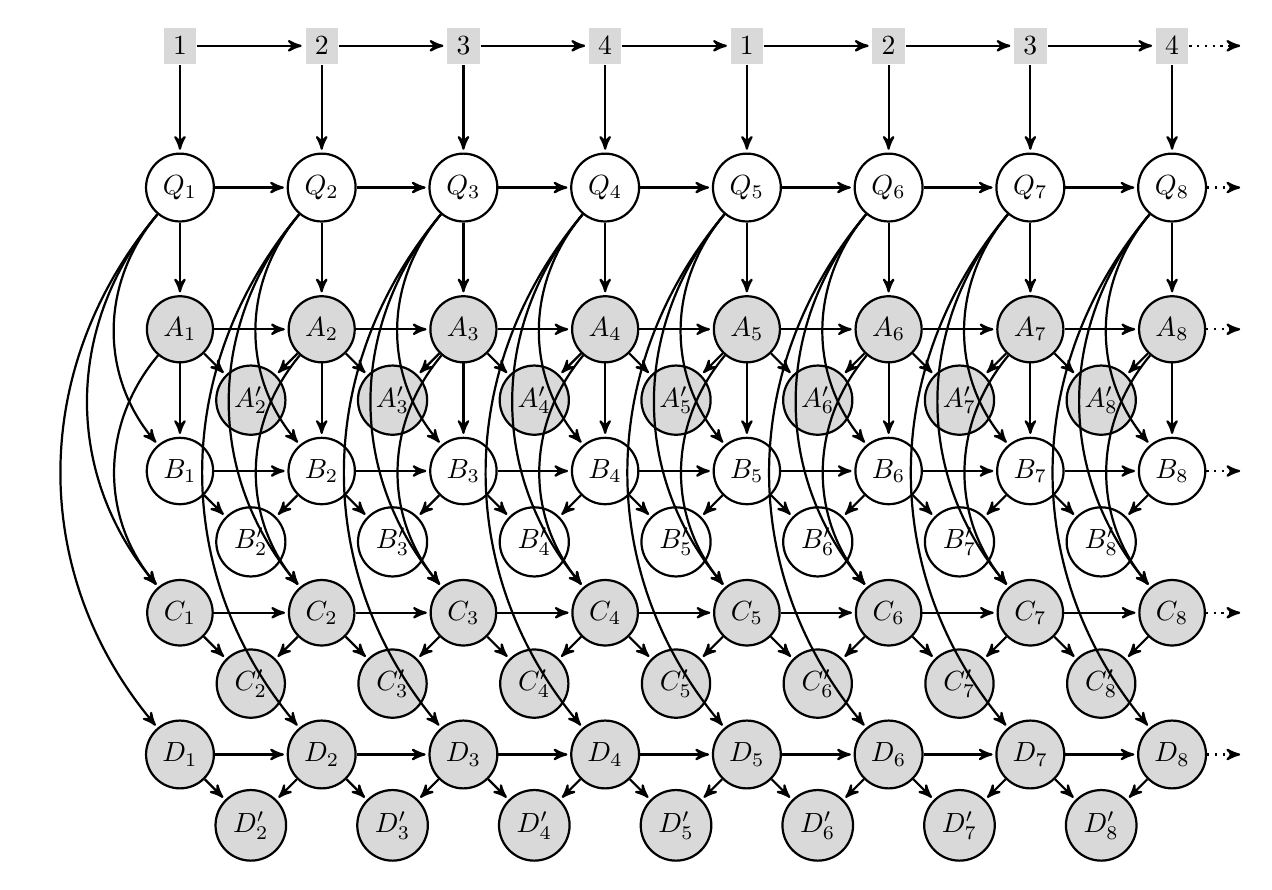
\begin{tikzpicture}[->, >=stealth',shorten >=1pt,auto, node distance=2cm, thick,main/.style={circle,draw}, x=1.8cm, y=1.8cm]
    % time
    \foreach \i in {1,...,4} {
        \node[rectangle, fill=gray!30] (t\i) at (\i,0) {$\i$};
    }
    \node[rectangle, fill=gray!30] (t5) at (5,0) {$1$};
    \node[rectangle, fill=gray!30] (t6) at (6,0) {$2$};
    \node[rectangle, fill=gray!30] (t7) at (7,0) {$3$};
    \node[rectangle, fill=gray!30] (t8) at (8,0) {$4$};
    
    % chords, notes
    \foreach \i in {1,...,8} {
        \node[main] (Q\i) at (\i,-1) {$Q_{\i}$};
        \node[main, fill=gray!30] (A\i) at (\i,-2) {$A_{\i}$};
        \node[main] (B\i) at (\i,-3) {$B_{\i}$};
        \node[main, fill=gray!30] (C\i) at (\i,-4) {$C_{\i}$};
        \node[main, fill=gray!30] (D\i) at (\i,-5) {$D_{\i}$};
    }
    \eat{
    \foreach \i in {1,...,7} {
        \node[main] (A'\i) at (\i.5, -2.5) {$A'_{\i}$};
        \draw (A\i) to (A'\i);
    }
    }
    \node[main, fill=gray!30] (A'2) at (1.5,-2.5) {$A'_{2}$};
    \node[main, fill=gray!30] (A'3) at (2.5,-2.5) {$A'_{3}$};
    \node[main, fill=gray!30] (A'4) at (3.5,-2.5) {$A'_{4}$};
    \node[main, fill=gray!30] (A'5) at (4.5,-2.5) {$A'_{5}$};
    \node[main, fill=gray!30] (A'6) at (5.5,-2.5) {$A'_{6}$};
    \node[main, fill=gray!30] (A'7) at (6.5,-2.5) {$A'_{7}$};
    \node[main, fill=gray!30] (A'8) at (7.5,-2.5) {$A'_{8}$};
    
    \node[main] (B'2) at (1.5,-3.5) {$B'_{2}$};
    \node[main] (B'3) at (2.5,-3.5) {$B'_{3}$};
    \node[main] (B'4) at (3.5,-3.5) {$B'_{4}$};
    \node[main] (B'5) at (4.5,-3.5) {$B'_{5}$};
    \node[main] (B'6) at (5.5,-3.5) {$B'_{6}$};
    \node[main] (B'7) at (6.5,-3.5) {$B'_{7}$};
    \node[main] (B'8) at (7.5,-3.5) {$B'_{8}$};
    
    \node[main, fill=gray!30] (C'2) at (1.5,-4.5) {$C'_{2}$};
    \node[main, fill=gray!30] (C'3) at (2.5,-4.5) {$C'_{3}$};
    \node[main, fill=gray!30] (C'4) at (3.5,-4.5) {$C'_{4}$};
    \node[main, fill=gray!30] (C'5) at (4.5,-4.5) {$C'_{5}$};
    \node[main, fill=gray!30] (C'6) at (5.5,-4.5) {$C'_{6}$};
    \node[main, fill=gray!30] (C'7) at (6.5,-4.5) {$C'_{7}$};
    \node[main, fill=gray!30] (C'8) at (7.5,-4.5) {$C'_{8}$};
    
    \node[main, fill=gray!30] (D'2) at (1.5,-5.5) {$D'_{2}$};
    \node[main, fill=gray!30] (D'3) at (2.5,-5.5) {$D'_{3}$};
    \node[main, fill=gray!30] (D'4) at (3.5,-5.5) {$D'_{4}$};
    \node[main, fill=gray!30] (D'5) at (4.5,-5.5) {$D'_{5}$};
    \node[main, fill=gray!30] (D'6) at (5.5,-5.5) {$D'_{6}$};
    \node[main, fill=gray!30] (D'7) at (6.5,-5.5) {$D'_{7}$};
    \node[main, fill=gray!30] (D'8) at (7.5,-5.5) {$D'_{8}$};
    \eat{
    \draw (A2) to (A'1);
    \draw (A3) to (A'2);
    \draw (A4) to (A'3);
    \draw (A5) to (A'4);
    \draw (A6) to (A'5);
    \draw (A7) to (A'6);
    \draw (A8) to (A'7);
    }
    
    \eat{
    \foreach \i in {1,...,7} {
        \node[main] (B'\i) at (\i.5, -3.5) {$B'_{\i}$};
        \draw (B\i) to (B'\i);
    }
    }
    \eat{
    \draw (B2) to (B'1);
    \draw (B3) to (B'2);
    \draw (B4) to (B'3);
    \draw (B5) to (B'4);
    \draw (B6) to (B'5);
    \draw (B7) to (B'6);
    \draw (B8) to (B'7);
    }
    
    \eat{
    \foreach \i in {1,...,7} {
        \node[main] (C'\i) at (\i.5, -4.5) {$C'_{\i}$};
        \draw (C\i) to (C'\i);
    }
    
    \foreach \i in {1,...,7} {
        \node[main] (D'\i) at (\i.5, -5.5) {$D'_{\i}$};
        \draw (D\i) to (D'\i);
    }
    }
    \foreach \a in {A,B,C,D} {
    \draw (\a2) to (\a'2); \draw (\a1) to (\a'2);
    \draw (\a3) to (\a'3); \draw (\a2) to (\a'3);
    \draw (\a4) to (\a'4); \draw (\a3) to (\a'4);
    \draw (\a5) to (\a'5); \draw (\a4) to (\a'5);
    \draw (\a6) to (\a'6); \draw (\a5) to (\a'6);
    \draw (\a7) to (\a'7); \draw (\a6) to (\a'7);
    \draw (\a8) to (\a'8); \draw (\a7) to (\a'8);
    }
    
    \foreach \i in {1,...,8} {
        \draw (t\i) to (Q\i);
        \draw (Q\i) to (A\i);
        \draw[bend right=40] (Q\i) to (B\i);
        \draw[bend right=40] (Q\i) to (C\i);
        \draw[bend right=40] (Q\i) to (D\i);
        \draw (A\i) to (B\i);
        \draw[bend right=40] (A\i) to (C\i);
        
    }
    
    \foreach \a in {A,B,C,D,Q, t} {
        \draw (\a1) to (\a2);
        \draw (\a2) to (\a3);
        \draw (\a3) to (\a4);
        \draw (\a4) to (\a5);
        \draw (\a5) to (\a6);
        \draw (\a6) to (\a7);
        \draw (\a7) to (\a8);
    }
    \draw[dotted] (t8) to (8.5,0);
    \draw[dotted] (A8) to (8.5,-2);
    \draw[dotted] (B8) to (8.5,-3);
    \draw[dotted] (C8) to (8.5,-4);
    \draw[dotted] (D8) to (8.5,-5);
    \draw[dotted] (Q8) to (8.5,-1);
\end{tikzpicture}}
\end{center}
\caption{Final model}
\end{figure}

\begin{figure}[ht]
\begin{tabular}{cc}
%\multicolumn{2}{c}{
%\includegraphics[width=0.45\textwidth]{simple2-sopranoONLY.png}
%}\\
%\multicolumn{2}{c}{Simple model 1}\\
\includegraphics[width=0.45\textwidth]{simple2-sopranoONLY.png}&
\includegraphics[width=0.45\textwidth]{simple6-int3}\\
Intermediate 1 & Intermediate 3\\
\includegraphics[width=0.45\textwidth]{vit8_confplot.png}&
\includegraphics[width=0.45\textwidth]{vit8_preds.png}\\
Viterbi8: chords played & Viterbi8: chords predicted
\end{tabular}
\caption{Confusion matrices between true chord and played chord}
\end{figure}

\begin{figure}[ht]
\begin{tabular}{cc}
\multicolumn{2}{c}{
\includegraphics[width=0.45\textwidth]{distr_simple.png}
}\\
\multicolumn{2}{c}{Simple models}\\
\includegraphics[width=0.45\textwidth]{distr_int.png}&\includegraphics[width=0.45\textwidth]{distr_vit.png}\\
Intermediate models & Viterbi models\\
\end{tabular}
\caption{Distributions}
\end{figure}

\clearpage
\section{Viterbi Algorithm}

We present the derivation of the Viterbi algorithm for the Final model. Derivations for the other models are similar.
Let \[f(t) := p(T_{1:t}, Q_{1:t}, A_{1:t}, A'_{2:t}, B_{1:t}, B'_{2:t}, C_{1:t}, C'_{2:t}, D_{1:t}, D'_{2:t}).\]
We would like to maximize $f(t)$ with respect to $Q_{1:t}, B_{1:t}, B'_{2:t}$. Note that
\[\max_{\substack{Q_{1:t},\\B_{1:t},\\B'_{2:t}}}f(t)=\max_{Q_t, B_t, B'_t}\max_{\substack{Q_{1:t-1},\\B_{1:t-1},\\B'_{2:t-1}}}f(t).\]
So, it suffices to find the inner maximum for every instance of $Q_t, B_t, B'_t$, and then take the maximum over these three variables.

Suppose by induction that we have already found $\alpha_{t-1}(Q_{t-1}, B_{t-1}, B'_{t-1}) := \max\limits_{\substack{Q_{1:t-2},\\ B_{1:t-2}\\B'_{2:t-2}}} f(t-1)$. Using the conditional independence assumptions in the model, we have
\begin{tiny}
\begin{align*}
\alpha_t(Q_t, B_t, B'_t) &:=
\max\limits_{\substack{Q_{1:t-1},\\ B_{1:t-1},\\B'_{2:t-1}}} f(t)\\ 
&= \max\limits_{\substack{Q_{1:t-1},\\ B_{1:t-1},\\B'_{2:t-1}}} p(T_{1:t}, Q_{1:t}, A_{1:t}, A'_{2:t}, B_{1:t}, B'_{2:t}, C_{1:t}, C'_{2:t}, D_{1:t}, D'_{2:t})\\
%&= \max\limits_{\substack{Q_{1:t-1},\\ A_{1:t-1}\\A'_{2:t-1}}}
%\left[
%p(T_t, Q_t, A_t, A'_t, B_t, B'_t, C_t, C'_t, D_t, D'_t \mid T_{1:t-1}, Q_{1:t-1}, A_{1:t-1}, A'_{2:t-1}, B_{1:t-1},B'_{2:t-1}, C_{1:t-1},C'_{2:t-1}, D_{1:t-1}, D'_{1:t-1} ) p(T_{1:t-1}, Q_{1:t-1}, A_{1:t-1}, A'_{2:t-1}, B_{1:t-1},B'_{2:t-1}, C_{1:t-1},C'_{2:t-1}, D_{1:t-1}, D'_{1:t-1})
%\right]\\
%\intertext{By Baye's ball,}
%\intertext{Using conditional independence,}
&= \max\limits_{\substack{Q_{1:t-1},\\ A_{1:t-1},\\A'_{2:t-1}}}
\left[
p(T_t, Q_t, A_t, A'_t, B_t, B'_t, C_t, C'_t, D_t, D'_t \mid T_{t-1}, Q_{t-1}, A_{t-1}, B_{t-1}, C_{t-1} ) f(t-1)
\right]\\
&= \max\limits_{\substack{Q_{t-1},\\ B_{t-1},\\B'_{t-1}}} \max\limits_{\substack{Q_{1:t-2},\\ B_{1:t-2},\\B'_{2:t-2}}}
\Bigg[
p(T_t \mid T_{t-1})
p(Q_t \mid Q_{t-1}, T_t)\\&\qquad\qquad
p(A_t \mid A_{t-1}, Q_t)
p(B_t \mid B_{t-1}, Q_t, A_t)
p(C_t \mid C_{t-1}, Q_t, A_t)
p(D_t \mid D_{t-1}, Q_t)\\&\qquad\qquad
p(A'_t \mid A_{t-1}, A_t)
p(B'_t \mid B_{t-1}, B_t)
p(C'_t \mid C_{t-1}, C_t)
p(D'_t \mid D_{t-1}, D_t)
f(t-1)\Bigg]\\
%&= \max\limits_{\substack{Q_{t-1},\\ A_{t-1}}}
%\left[
%p(Q_t \mid Q_{t-1}, T_t)
%p(A_t \mid A_{t-1}, Q_t)
%p(B_t \mid B_{t-1}, Q_t)
%p(C_t \mid C_{t-1}, Q_t)
% \max\limits_{\substack{Q_{1:t-2},\\ A_{1:t-2}}} f(t-1)
% \right]\\
&= \max\limits_{\substack{Q_{t-1},\\ B_{t-1},\\B'_{t-1}}} 
\Bigg[
p(T_t \mid T_{t-1})
p(Q_t \mid Q_{t-1}, T_t)\\&\qquad\qquad
p(A_t \mid A_{t-1}, Q_t)
p(B_t \mid B_{t-1}, Q_t, A_t)
p(C_t \mid C_{t-1}, Q_t, A_t)
p(D_t \mid D_{t-1}, Q_t)\\&\qquad\qquad
p(A'_t \mid A_{t-1}, A_t)
p(B'_t \mid B_{t-1}, B_t)
p(C'_t \mid C_{t-1}, C_t)
p(D'_t \mid D_{t-1}, D_t)
\max\limits_{\substack{Q_{1:t-2},\\ B_{1:t-2},\\B'_{2:t-2}}}
f(t-1)\Bigg]\\
%&= \max\limits_{\substack{Q_{t-1},\\ A_{t-1}}}
%\left[
%p(Q_t \mid Q_{t-1}, T_t)
%p(A_t \mid A_{t-1}, Q_t)
%p(B_t \mid B_{t-1}, Q_t)
%p(C_t \mid C_{t-1}, Q_t)
%\alpha_{t-1}
% \right]
&= \max\limits_{\substack{Q_{t-1},\\ B_{t-1},\\B'_{t-1}}} 
\Bigg[
p(T_t \mid T_{t-1})
p(Q_t \mid Q_{t-1}, T_t)
p(A_t \mid A_{t-1}, Q_t)\\&\qquad\qquad
p(B_t \mid B_{t-1}, Q_t, A_t)
p(C_t \mid C_{t-1}, Q_t, A_t)
p(D_t \mid D_{t-1}, Q_t)
p(A'_t \mid A_{t-1}, A_t)\\&\qquad\qquad
p(B'_t \mid B_{t-1}, B_t)
p(C'_t \mid C_{t-1}, C_t)
p(D'_t \mid D_{t-1}, D_t)
\alpha_{t-1}(Q_{t-1}, B_{t-1}, B'_{t-1})\Bigg]\\
\end{align*}
\end{tiny}

Note that in the base case $t=1$, we have
    \[
    \max\limits_{\substack{Q_{1:0},\\ B_{1:0}}} p(T_1,Q_1, A_1, B_1, C_1, D_1) = p(T_1) p(Q_1 \mid T_1) p(A_1 \mid Q_1) p(B_1 \mid Q_1, A_1) p(C_1 \mid Q_1, A_1) p(D_1 \mid Q_1).
    \]




\eat{
\resizebox{0.5\textwidth}{!}{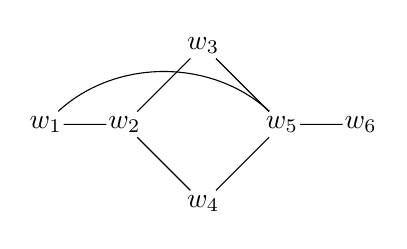
\begin{tikzpicture}[baseline=-0.5ex]
    \draw (0,0) -- (1,0) -- (2,1) -- (3,0) -- (4,0);
    \draw (1,0) -- (2,-1) -- (3,0);
    \draw[bend left = 50] (0,0) to (3,0);
    \node[star] at (0,0) {$w_1$};
    \node[star] at (1,0) {$w_2$};
    \node[star] at (2,1) {$w_3$};
    \node[star] at (2,-1) {$w_4$};
    \node[star] at (3,0) {$w_5$};
    \node[star] at (4,0) {$w_6$};
\end{tikzpicture}}

\begin{center}\resizebox{0.5\textwidth}{!}{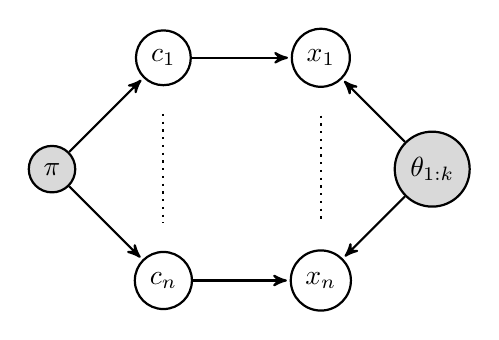
\begin{tikzpicture}[->, >=stealth',shorten >=1pt,auto, node distance=2cm, thick,main/.style={circle,draw}]

  \node[main, fill=gray!30] (pi) {$\pi$};
  \node[main] (c1) [above right of =pi]{$c_1$};
  \node[main] (cn) [below right of =pi]{$c_n$};
  \node[main] (x1) [right of = c1]{$x_1$}; 
  \node[main] (xn) [right of = cn]{$x_n$};
  \node[main, fill=gray!30] (theta) [below right of = x1]{$\theta_{1:k}$};
  \path
    (pi) edge (c1) edge (cn)
    (c1) edge (x1)
    (cn) edge (xn)
    (theta) edge (x1) edge (xn)
    ;
   \path[dotted, -, shorten >= 10pt, shorten <= 10pt]
    (c1) edge (cn)
    (x1) edge (xn)
    ;
\end{tikzpicture}}\end{center}
}
\eat{
\begin{verbatim}
let M be the total number of timesteps (quarter notes)
let S be the total number of triplets (Q_t, A_t, A'_t)
keep a M x S array for "best previous state"
keep a M x S array for "maximum probability"
initialize first timestep using base case (will have redundancy with eighth note)
for each time step t
    for each triplet (Q_t, A_t, A'_t)
        for each triplet (Q_{t-1}, A_{t-1}, A'_{t-1})
            compute probability (last line of long calculation above),
            keep track of max
        store max in "maximum probability" array
        store best previous state in "best previous state" array
for last time step M, compute maximum (over all triplets (Q_M, A_M, A'_M))
recover best sequence by backtracking through "best previous state" array
\end{verbatim}
}


\end{small}
\end{document}
